%%% The main file. It contains definitions of basic parameters and includes all other parts.

%% Settings for single-side (simplex) printing
% Margins: left 40mm, right 25mm, top and bottom 25mm
% (but beware, LaTeX adds 1in implicitly)
\documentclass[12pt,a4paper]{report}
\setlength\textwidth{145mm}
\setlength\textheight{247mm}
\setlength\oddsidemargin{15mm}
\setlength\evensidemargin{15mm}
\setlength\topmargin{0mm}
\setlength\headsep{0mm}
\setlength\headheight{0mm}
% \openright makes the following text appear on a right-hand page
\let\openright=\clearpage

%% Settings for two-sided (duplex) printing
% \documentclass[12pt,a4paper,twoside,openright]{report}
% \setlength\textwidth{145mm}
% \setlength\textheight{247mm}
% \setlength\oddsidemargin{14.2mm}
% \setlength\evensidemargin{0mm}
% \setlength\topmargin{0mm}
% \setlength\headsep{0mm}
% \setlength\headheight{0mm}
% \let\openright=\cleardoublepage

%% Character encoding: usually latin2, cp1250 or utf8:
\usepackage[utf8]{inputenc}

%% Further useful packages (included in most LaTeX distributions)
\usepackage{amsmath}        % extensions for typesetting of math
\usepackage{amsfonts}       % math fonts
\usepackage{amsthm}         % theorems, definitions, etc.
\usepackage{bbding}         % various symbols (squares, asterisks, scissors, ...)
\usepackage{bm}             % boldface symbols (\bm)
\usepackage{graphicx}       % embedding of pictures
\usepackage{fancyvrb}       % improved verbatim environment
\usepackage{natbib}         % citation style AUTHOR (YEAR), or AUTHOR [NUMBER]
\usepackage[nottoc]{tocbibind} % makes sure that bibliography and the lists
			    % of figures/tables are included in the table
			    % of contents
\usepackage{dcolumn}        % improved alignment of table columns
\usepackage{booktabs}       % improved horizontal lines in tables
\usepackage{paralist}       % improved enumerate and itemize
\usepackage[usenames]{xcolor}  % typesetting in color
\usepackage{soul}           % HIGHLIGHTER
\usepackage{minted}         % code listings
\usepackage{tikz}           % pictures
\usepackage{pgfplots}       % charts

\usemintedstyle{xcode}      % syntax highlighting color pallette
\usetikzlibrary{shapes,matrix,chains,positioning,decorations.pathreplacing,arrows,hobby,decorations.markings,backgrounds}       % more libs

%%% Basic information on the thesis

% Thesis title in English (exactly as in the formal assignment)
\def\ThesisTitle{Genetic programming~in Swift for~human-competitive evolution}

% Author of the thesis
\def\ThesisAuthor{Petr~Mánek}

% Year when the thesis is submitted
\def\YearSubmitted{2016}

% Name of the department or institute, where the work was officially assigned
% (according to the Organizational Structure of MFF UK in English,
% or a full name of a department outside MFF)
\def\Department{Department of~Software and Computer~Science Education}

% Is it a department (katedra), or an institute (ústav)?
\def\DeptType{Department}

% Thesis supervisor: name, surname and titles
\def\Supervisor{RNDr. František~Mráz, CSc.}

% Supervisor's department (again according to Organizational structure of MFF)
\def\SupervisorsDepartment{Department of~Software and Computer~Science Education}

% Study programme and specialization
\def\StudyProgramme{Computer~Science}
\def\StudyBranch{General Computer~Science}

% An optional dedication: you can thank whomever you wish (your supervisor,
% consultant, a person who lent the software, etc.)
\def\Dedication{%todo
Dedication.
}

% Abstract (recommended length around 80-200 words; this is not a copy of your thesis assignment!)
\def\Abstract{
Imitating the process of natural selection, evolutionary algorithms have shown to be efficient search techniques for optimization and machine learning in poorly understood and irregular spaces. In this thesis, we implement a library containing essential implementation of such algorithms in recently unveiled programming language Swift. The result is a lightweight framework compatible with Linux-based computing clusters as well as mobile devices. Such wide range of supported platforms allows for successful application even in situations, where signals from various sensors have to be acquired and processed independently of other devices. In addition, thanks to Swift's minimalistic and functional syntax, the implementation of bundled algorithms and their sample usage clearly demonstrates fundamentals of genetic programming, making the work usable in teaching and quick prototyping of evolutionary algorithms. 
}

% 3 to 5 keywords (recommended), each enclosed in curly braces
\def\Keywords{
{genetic} {programming}
{artificial} {evolution}
}

%% The hyperref package for clickable links in PDF and also for storing
%% metadata to PDF (including the table of contents).
\usepackage[pdftex,unicode]{hyperref}   % Must follow all other packages
\hypersetup{breaklinks=true}
\hypersetup{pdftitle={\ThesisTitle}}
\hypersetup{pdfauthor={\ThesisAuthor}}
\hypersetup{pdfkeywords=\Keywords}
\hypersetup{urlcolor=blue}

% Definitions of macros (see description inside)
%%% This file contains definitions of various useful macros and environments %%%
%%% Please add more macros here instead of cluttering other files with them. %%%

%%% Minor tweaks of style

% These macros employ a little dirty trick to convince LaTeX to typeset
% chapter headings sanely, without lots of empty space above them.
% Feel free to ignore.
\makeatletter
\def\@makechapterhead#1{
  {\parindent \z@ \raggedright \normalfont
   \Huge\bfseries \thechapter. #1
   \par\nobreak
   \vskip 20\p@
}}
\def\@makeschapterhead#1{
  {\parindent \z@ \raggedright \normalfont
   \Huge\bfseries #1
   \par\nobreak
   \vskip 20\p@
}}
\makeatother

% This macro defines a chapter, which is not numbered, but is included
% in the table of contents.
\def\chapwithtoc#1{
\chapter*{#1}
\addcontentsline{toc}{chapter}{#1}
}

% Draw black "slugs" whenever a line overflows, so that we can spot it easily.
\overfullrule=1mm

%%% Macros for definitions, theorems, claims, examples, ... (requires amsthm package)

\theoremstyle{plain}
\newtheorem{thm}{Theorem}
\newtheorem{lemma}[thm]{Lemma}
\newtheorem{claim}[thm]{Claim}

\theoremstyle{plain}
\newtheorem{defn}{Definition}

\theoremstyle{remark}
\newtheorem*{cor}{Corollary}
\newtheorem*{rem}{Remark}
\newtheorem*{example}{Example}

%%% An environment for proofs

%%% FIXME %%% \newenvironment{proof}{
%%% FIXME %%%   \par\medskip\noindent
%%% FIXME %%%   \textit{Proof}.
%%% FIXME %%% }{
%%% FIXME %%% \newline
%%% FIXME %%% \rightline{$\square$}  % or \SquareCastShadowBottomRight from bbding package
%%% FIXME %%% }

%%% An environment for typesetting of program code and input/output
%%% of programs. (Requires the fancyvrb package -- fancy verbatim.)

\DefineVerbatimEnvironment{code}{Verbatim}{fontsize=\small, frame=single}

%%% The field of all real and natural numbers
\newcommand{\R}{\mathbb{R}}
\newcommand{\N}{\mathbb{N}}

%%% Useful operators for statistics and probability
\DeclareMathOperator{\pr}{\textsf{P}}
\DeclareMathOperator{\E}{\textsf{E}\,}
\DeclareMathOperator{\var}{\textrm{var}}
\DeclareMathOperator{\sd}{\textrm{sd}}

%%% Transposition of a vector/matrix
\newcommand{\T}[1]{#1^\top}

%%% Various math goodies
\newcommand{\goto}{\rightarrow}
\newcommand{\gotop}{\stackrel{P}{\longrightarrow}}
\newcommand{\maon}[1]{o(n^{#1})}
\newcommand{\abs}[1]{\left|{#1}\right|}
\newcommand{\dint}{\int_0^\tau\!\!\int_0^\tau}
\newcommand{\isqr}[1]{\frac{1}{\sqrt{#1}}}

%%% Various table goodies
\newcommand{\pulrad}[1]{\raisebox{1.5ex}[0pt]{#1}}
\newcommand{\mc}[1]{\multicolumn{1}{c}{#1}}



%%% Custom PM macros
\newcommand*{\todo}{\hl{\textbf{TODO}}}
\newcommand{\inputswift}[1]{\inputminted[linenos,
               numbersep=5pt,
               frame=lines,
               framesep=2mm,
               fontsize=\small]{swift}{code/#1.swift}}


% Title page and various mandatory informational pages
\begin{document}
%%% Title page of the thesis and other mandatory pages

%%% Title page of the thesis

\pagestyle{empty}
\hypersetup{pageanchor=false}
\begin{center}

\large

Charles University in Prague

\medskip

Faculty of Mathematics and Physics

\vfill

{\bf\Large BACHELOR THESIS}

\vfill

\centerline{\mbox{
\includegraphics[width=60mm]{img/logo.pdf}}}

\vfill
\vspace{5mm}

{\LARGE\ThesisAuthor}

\vspace{15mm}

{\LARGE\bfseries\ThesisTitle}

\vfill

\Department

\vfill

\begin{tabular}{rl}

Supervisor of the bachelor thesis: & \Supervisor \\
\noalign{\vspace{2mm}}
Study programme: & \StudyProgramme \\
\noalign{\vspace{2mm}}
Study branch: & \StudyBranch \\
\end{tabular}

\vfill

% Zde doplňte rok
Prague \YearSubmitted

\end{center}

\newpage

%%% Here should be a bound sheet included -- a signed copy of the "bachelor
%%% thesis assignment". This assignment is NOT a part of the electronic
%%% version of the thesis. DO NOT SCAN.

%%% A page with a solemn declaration to the bachelor thesis

\openright
\hypersetup{pageanchor=true}
\pagestyle{plain}
\pagenumbering{roman}
\vglue 0pt plus 1fill

\noindent
I declare that I carried out this bachelor thesis independently, and only with the cited
sources, literature and other professional sources.

\medskip\noindent
I understand that my work relates to the rights and obligations under the Act No.~121/2000 Sb.,
the Copyright Act, as amended, in particular the fact that the Charles
University in Prague has the right to conclude a license agreement on the use of this
work as a school work pursuant to Section 60 subsection 1 of the Copyright Act.

\vspace{10mm}

\hbox{\hbox to 0.5\hsize{%
In ........ date ............	% FIXME!
\hss}\hbox to 0.5\hsize{%
signature of the author
\hss}}

\vspace{20mm}
\newpage

%%% Mandatory information page of the thesis

\openright

\vbox to 0.5\vsize{
\setlength\parindent{0mm}
\setlength\parskip{5mm}

Title:
\ThesisTitle

Author:
\ThesisAuthor

\DeptType:
\Department

Supervisor:
\Supervisor, \SupervisorsDepartment

Abstract:
\Abstract

Keywords:
\Keywords

\vss}

\newpage

%%% Dedication

\openright

\noindent
\Dedication

\newpage

\openright
\pagestyle{plain}
\pagenumbering{arabic}
\setcounter{page}{1}


%%% A page with automatically generated table of contents of the bachelor thesis

\tableofcontents

%%% Each chapter is kept in a separate file
\chapter{Introduction}

\section{Genetic Algorithms}
Genetic algorithms (GA) are iterative randomized optimization methods\footnote{In this work, genetic algorithms are equivalent to \textit{generational models} defined in \cite{AdaptationInSystems}.}, which are inspired by the biological process of natural selection. In the context of GA, points in the domain space are represented to \textit{individuals} of animal species. Every individual carries a \textit{chromosome}, which describes its location in the domain space, thus defining its properties similarly to the way DNA defines skills and capabilities of its carriers.

To initialize the GA, a \textit{population} of individuals with random chromosomes is generated. During single iteration of the GA, individuals in the population compete for their right to reproduce, favoring those who maximize the value of a \textit{fitness function} which customarily maps every individual to a single decimal value from the $[0;1]$ interval. At the end of the iteration, fit individuals are selected and allowed to produce an \textit{offspring population}, on which the next iteration of the GA operates. This behavior creates an iterative loop, which can be summarized by a diagram shown in Figure \ref{fig:genetic-flowchart}.

\begin{figure}[ht]
	\centering
	\scriptsize
	\begin{tikzpicture}[
		node distance = 1.5cm, 
		auto,
		decision/.style={
			diamond, 
			draw, 
    		text width=5em, 
    		text badly centered, 
    		node distance=2cm, 
    		inner sep=0pt
    		},
		block/.style={
			rectangle, 
			draw, 
			text width=6.5em, 
			text centered, 
			minimum height=4em
			},
		line/.style={
			draw,
			-latex'
			}]
	    % Place nodes
	    \node [block] (init) {Generate random population.};
	    \node [block, below of=init] (evaluate2) {Evaluate\\population.};
	    \node [decision, below of=evaluate2] (termination) {Should terminate?};
	    \node [block, below of=termination, node distance=2cm] (reset) {Reset\\offspring.};
	    \node [block, right of=termination, node distance=3cm] (stop) {Terminate.};
	    \node [decision, below of=reset] (enough) {Have enough offpring?};

	    \node [block, below of=enough, node distance=2.3cm] (operator) {Choose genetic operator.};
	    \node [block, left of=enough, node distance=3cm] (evaluate) {Evaluate\\offspring.};
	    \node [block, above of=evaluate, node distance=2cm] (swap) {Swap\\generations.};
	    \node [block, right of=operator, node distance=3cm] (insert) {Insert\\offspring\\ individual.};

	    % Draw edges
	    \path [line] (init) -- (evaluate2);
	    \path [line] (evaluate2) -- (termination);
	    \path [line] (termination) -- node {no}(reset);
	    \path [line] (reset) -- (enough);
	    \path [line] (enough) -- node {no}(operator);
	    \path [line] (enough) -- node {yes}(evaluate);
	    \path [line] (evaluate) -- (swap);
	    \path [line] (swap) |- (termination);
	    \path [line] (termination) -- node {yes}(stop);
	    \path [line] (operator) -- (insert);
	    \path [line] (insert) |- (enough);
	\end{tikzpicture}

	\caption{Generalized decision diagram of a GA.}
	\label{fig:genetic-flowchart}
\end{figure}

Although there are many variants of GA, each with different properties and applications, the basic notion stays the same. Genetic algorithms iteratively evaluate and modify a population of chromosomes until a set \textit{termination condition} met. This condition can for instance ascertain the fitness of the best chromosome so far or simply count the number of iterations performed. Individuals are inserted in the population at two instances throughout the execution of the GA: first during the initialization when a random population is generated, and second when the population is modified to prepare grounds for the next iteration. The latter of the two is the key phase of the GA. At this point in execution, the algorithm explores new points of the domain space by reusing points which have already been discovered. Such process is often based on non-deterministic inputs and can utilize the fitness of the chromosomes discovered so far as a heuristic. Instances of this process are referred to as \textit{genetic operators}.

The \textit{selection pressure} is the degree to which the better individuals are favored: the higher the selection pressure, the more the better individuals are favored. This selection pressure drives the GA to improve the population fitness over succeeding generations. However, if the selection pressure is too low, the convergence rate will be slow, and the GA will unnecessarily take longer to find the optimal solution. If the selection pressure is too high, there is an increased chance of the genetic algorithm prematurely converging to an incorrect (suboptimal) solution. \cite{GaTournamentSelection}

\section{Neural Networks}\label{section:neural-networks}
A neural network is an interconnected assembly of simple processing elements, \textit{units} or \textit{nodes}, whose functionality is loosely based on the animal neuron. The processing ability of the network is stored in the interunit connection strengths, or \textit{weights}, obtained by a process of adaptation to, or \textit{learning} from a set of training patterns. \cite{NeuralNets}

A neural network is called \textit{feedforward} (denoted FFNN), if its interunit connections do not form a cycle. In such case, it makes sense to clasify its nodes in separate \textit{layers} with respect to their topological ordering. The first layer of the network is customarily called the \textit{input layer}, whereas the last layer is called the \textit{output layer}. The remaining layers are referred to as the \textit{hidden layers}. This is illustrated in Figure \ref{fig:FFNN}.

\begin{figure}[ht]
	\centering
	\scriptsize
	\begin{tikzpicture}[
		plain/.style={
		  draw=none,
		  fill=none,
		  },
		net/.style={
		  matrix of nodes,
		  nodes={
		    draw,
		    circle,
		    inner sep=7pt
		    },
		  nodes in empty cells,
		  column sep=1cm,
		  row sep=-9pt
		  },
		>=latex
		]
		\matrix[net] (mat)
		{
		|[plain]| \parbox{1.3cm}{\centering Input\\layer} & |[plain]| \parbox{1.3cm}{\centering Hidden\\layer} & |[plain]| \parbox{1.3cm}{\centering Output\\layer} \\
		& |[plain]| \\
		|[plain]| & \\
		& |[plain]| \\
		|[plain]| & |[plain]| \\
		& & \\
		|[plain]| & |[plain]| \\
		& |[plain]| \\
		|[plain]| & \\
		& |[plain]| \\
		};
		\foreach \ai [count=\mi ]in {2,4,...,10}
		  \draw[<-] (mat-\ai-1) -- node[above] {Input \mi} +(-2cm,0);
		\foreach \ai in {2,4,...,10}
		{\foreach \aii in {3,6,9}
		  \draw[->] (mat-\ai-1) -- (mat-\aii-2);
		}
		\foreach \ai in {3,6,9}
		  \draw[->] (mat-\ai-2) -- (mat-6-3);
		\draw[->] (mat-6-3) -- node[above] {Output} +(2cm,0);
	\end{tikzpicture}
	\caption[A feedforward neural network.]{A feedforward neural network comprised of three layers of nodes.}
	\label{fig:FFNN}
\end{figure}

\subsection{Mathematical Representation}
In feedforward neural networks, signals travel between connected nodes in a way resembling the action potential of biological neural systems. Firstly, nodes of the input layer are evaluated with real numbers. From these values, the nodes of the second layer calculate their outputs, then the nodes of the third layer calculate their outputs based on the outputs of the second layer, and so on. This process propagates through the rest of the network until the output layer is reached. Since there are no cycles in the interunit connections of the FFNN, a finite number of steps is required to achieve such state. The outputs of the nodes located in the output layer are considered to be the outputs of the neural network. By this description, it is possible to think of the FFNN as a real vector function from $m$-dimensional to $n$-dimensional space, where $m,n$ denote the number of nodes in the input and the output layer respectively.

The process of calculating the output of a single node with respect to its inputs (which are in fact the outputs of the nodes of the previous layer) is quite straightforward. The output is defined as
~
\begin{align}
	y = f\left(b+\sum_{i=1}^n w_i x_i\right)
\end{align}
~
where $\{x_i\}_{i=1}^n$ denote the input values, $\{w_i\}_{i=1}^n$ denote the interunit connection weights, $b$ denotes the \textit{bias parameter} of the node and $f$ denotes the \textit{activation function}. The combination of all these parameters is illustrated in Figure \ref{fig:neuron-combination}.

\begin{figure}[ht]
	\centering
	\scriptsize
	\begin{tikzpicture}[
		init/.style={
		  draw,
		  circle,
		  inner sep=2pt,
		  font=\Huge,
		  join = by -latex
		},
		squa/.style={
		  draw,
		  inner sep=2pt,
		  font=\Large,
		  join = by -latex
		},
		start chain=2,node distance=13mm
		]
		\node[on chain=2] 
		  (x2) {$x_2$};
		\node[on chain=2,join=by o-latex] 
		  {$w_2$};
		\node[on chain=2,init] (sigma) 
		  {$\displaystyle\Sigma$};
		\node[on chain=2,squa,label=above:{\parbox{2cm}{\centering Activation \\ function}}]   
		  {$f$};
		\node[on chain=2,label=above:Output,join=by -latex] 
		  {$y$};
		\begin{scope}[start chain=1]
		\node[on chain=1] at (0,1cm) 
		  (x1) {$x_1$};
		\node[on chain=1,join=by o-latex] 
		  (w1) {$w_1$};
		\end{scope}
		\begin{scope}[start chain=3]
		\node[on chain=3] at (0,-1cm) 
		  (x3) {$x_3$};
		\node[on chain=3,label=below:Weights,join=by o-latex] 
		  (w3) {$w_3$};
		\end{scope}
		\node[label=above:\parbox{2cm}{\centering Bias \\ $b$}] at (sigma|-w1) (b) {};

		\draw[-latex] (w1) -- (sigma);
		\draw[-latex] (w3) -- (sigma);
		\draw[o-latex] (b) -- (sigma);

		\draw[decorate,decoration={brace,mirror}] (x1.north west) -- node[left=10pt] {Inputs} (x3.south west);
	\end{tikzpicture}

	\caption[A diagram of FFNN node evaluation.]{A diagram of FFNN node evaluation with three inputs.}
	\label{fig:neuron-combination}
\end{figure}

It is worth noting at this point that a constant number of weights can be achieved by assigning non-existant interunit connections zero weights. For the purposes of implementation, it is also possible to approximate the effects of the bias parameter by creating one additional node in every layer and configuring it to produce constant output. The bias of every node in the layer is then simply encoded into connection weights of such node.

\section{The Swift Programming Language}
In 2014, the Apple Corporation in California unveiled a new programming language called \textit{Swift}. \cite{SwiftReference} This language has been since then widely adopted by software developers and computer engineers, succeeding Objective-C as the main programming language used for application development on the Apple platform. Building on proven coding paradigms, such as generics and strongly-typed objects, Swift strives to be a modern, concise and safe alternative to popular languages like Python or C++ while attempting to maintain comparable performance in terms of computational speed and memory management (this has been observed experimentally \cite{PrimateLabsBenchmark}).

The latest version of the language is called \textit{Swift 2.2}. Announced at the World Wide Developer Conference in 2015, the new Swift extended minimalistic syntax of its predecessor to include error handling, condition assertion and instruction deferring. It also enables developers to create \textit{frameworks}, redistributable packages containing documentation and binary libraries that other developers can include and utilize in their projects.

Since Fall 2015, Swift along with its standard library\footnote{The Swift standard library is comprised of two main components, the \textit{Foundation} module and the \textit{libdispatch} scheduling library.} became an open-source project, integrating itself into the LLVM (Low-level Virtual Machine), a widely-used compiler compatible with thousands of devices running Linux-based operating systems. Thanks to these modifications, Swift has been lately discussed as an attractive option for academic collaborations and community-driven projects.

\section{Analysis}
\todo

\section{Structure of This Document}
For the reader's convenience, this section contains a brief description of the rest of this thesis.

Chapter 2 provides details on the object design of the presented library. It introduces its individual components, explains their purpose and gives recommendations on their usage. In addition, the chapter includes short Swift code fragments to further illustrate some referenced programming techniques.

Chapter 3 is dedicated to practical usage demonstrations of the library as a whole. It contains three demonstrations selected from a broader list of example projects which are part of the library source package. In the first demonstration, a trivial abstract problem is solved with GA. The goal of the second demonstration is to train a real-time car-driving software based on FFNN. The third demonstration attempts to partially replicate results presented in \cite{EvolvingQwopGaits}.

Chapter 4 contains the conclusion of this thesis. It summarizes its objectives, states its accomplishments and concludes by suggesting potential applications of the library in research, portable devices and teaching.

Appendix A is a survey of other GA libraries, conducted in September 2015 as a part of preliminary specification, which eventually led to the writing of this work.

The digital version of this thesis also contains Appendix B, which contains the library source package with implementation, unit tests, documentation and example projects.

\chapter{Background}
This chapter is dedicated to establishing and describing terms needed to understand the rest of the work.

\section{Genetic Algorithms}
Genetic algorithms (GA) are iterative randomized optimization techniques, which are inspired by the process of natural selection. In the context of GA, points in the domain space are likened to \textit{individuals} of a biological species. Every individual carries a \textit{chromosome}, which describes its location in the domain space, thus defining its properties and capabilities.

To initialize the GA, a \textit{population} of individuals with random chromosomes is generated. During single iteration of the GA, individuals in the population compete for their right to reproduce, favoring those who maximize the value of a \textit{fitness function} which customarily maps every individual to a value from the $[0;1]$ interval. At the end of the iteration, fit individuals are selected and allowed to produce an \textit{offspring population}, on which the next iteration of the GA operates.

\textit{The selection pressure} is the degree to which the better individuals are favored: the higher the selection pressure, the more the better individuals are favored. This selection pressure drives the GA to improve the population fitness over succeeding generations. However, if the selection pressure is too low, the convergence rate will be slow, and the GA will unnecessarily take longer to find the optimal solution. If the selection pressure is too high, there is an increased chance of the genetic algorithm prematurely converging to an incorrect (suboptimal) solution. \cite{GaTournamentSelection}

\section{Redistributable Applications}
\todo

\section{Analysis}
\todo

\section{Requirements}
\todo

% \chapter{Object-oriented Design}
% In this chapter, the high-level design of individual components of the library is described.

% \cite{Koza1992}
% \todo % odebrat toto, jakmile někde bude citace


% \section{Random Genereration}
% Randomness plays a crucial role in evolutionary algorithms. Since the properties of pseudo-random generators impact the quality of produced solutions significantly, the library gives users full control over the algorithm, which is used to produce random sequences. In object design, this is achieved by simple abstraction.

% The functionality of a random number generator is facilitated by \textit{an entropy generator} object. In runtime, only a single instance of such object is created. This instance is then passed on to other components of the library, which require its capabilities. These components access the entropy generator by reference. Users are responsible for instantiating this object, and can thus specify a seed for the generator or choose an algorithm particularly suitable for their application.

% For the sake of minimality, entropy generators are only required to produce positive floating-point decimals from the $[0;1]$ interval. In spite of that, they can be used to generate random values of various types. This mechanism provided that the generated decimals can be mapped onto the type while maintaining uniform distribution of generated values. This is further discussed in section \ref{section:data-structures}.


% \subsection{Data Structures}\label{section:data-structures}
% Every individual in a generation is repesented by a separate instance of a class. The primary responsibility of such object is to store genetic information, which defines the individual. This information does not need to be held in a homogeneous data structure. In fact, it can be stored in any type suitable for the application. The only requirement on such type is that it can be generated randomly.



% \todo

% \subsection{Randomizable Interface}
% \todo

% \subsection{Discrete Interface}
% \todo

% \section{Genetic Operators}
% \todo

% \subsection{Operator Life Cycle}
% \todo

% \subsection{Custom Interfaces}
% \todo

% \section{Selections}
% \todo

% \section{Algorithms}
% \todo

\chapter{Library Documentation}
This chapter contains technical documentation of individual components of the library, as well as examples of their usage.

\section{Chromosomes}
In the context of GA, \textit{a chromosome} (also known as \textit{genotype}) is a piece of information describing a solution to a problem. Since the nature and representation of such information heavily depends on the application, the library allows full customization of the underlying data structures, which are used to hold chromosomes. The library also provides implementation of some of the most frequently used structures, leaving users free to decide, whether to use a structure supplied by the library, implement a custom one, or combine multiple data structures together.

Within the library, chromosomes can be represented by any reference types, which conform to the \texttt{ChromosomeType} protocol. This protocol requires them to
~
\begin{enumerate}
	\item be immutable,\footnote{This is a semantical requirement implying that every chromosome modification will require a new instance of the type to be created.}
	\item be capable of randomly generating new instances.\footnote{This is achieved by requiring conformance to the \texttt{Randomizable} protocol.}
\end{enumerate}

This section explains, how to achieve common configurations using preimplemented types, how to customize them for different applications, and how to define custom data types for storing proprietary information.

\subsection{Data Representation Problem}
When designing chromosome data structures, users first need to decide which information should be stored within chromosomes and how should such information be encoded into primitive types. These questions might not always be trivial to answer and it is possible to show that 
unfortunate choices could potentially impact the rate of convergence of the GA significantly. This is known as \textit{the problem of data representation}.

It is worth noting at this point that the complexity of this problem extends far beyond the scope of this work, and is thus not addressed. For more information on this topic, readers are referred to ???. \todo

\subsection{Strings}\label{section:strings}
One of the most common ways of storing chromosomes is to encode them as strings of values of a same type, e. g. binary or numeric. Such strings are represented by \textit{range-initalized arrays}.

A range-initialized array is similar to a regular array in many ways. It is a generic list structure, which is capable of holding finite amounts of ordered homogeneous items. However, at the time of initialization, the number of elements in the array is set to a value, which non-deterministically selected from a given number interval. This allows for more flexibility, since in some applications, it is beneficial to vary not only the contents of the chromosome, but also its size. If this behavior is not required, the array can be configured to a constant length by using any interval of length zero.

A simple usage of range-initialized arrays can be demonstrated on the Knapsack Problem. Suppose that there are 10 things of different sizes and values and a knapsack of a limited capacity. The objective is to select things in order to maximize the total value of knapsack contents, while not exceeeding its capacity. All solutions of this problem can be described as strings of 10 Boolean values, indicating whether items 1-10 are selected. These values can be stored in a range-initialized array with interval $[10;10]$ (implying that the array has fixed size 10), which is declared in Listing \ref{listing:array-knapsack}.

\begin{listing}[ht]
	\inputswift{array-knapsack}
	\caption{Range-initialized array used to solve the Knapsack problem.}
	\label{listing:array-knapsack}
\end{listing}

In a similar way, range-initialized arrays can store integers to encode number sequences or floating-point decimals to describe connection weights of neural networks. Thanks to Swift extensions, every instance of range-initialized array automatically conforms to the \texttt{ChromosomeType} protocol and supports three basic genetic operators (for definition, see section \ref{section:genetic-operators}). Range-initialized arrays can thus be directly used as chromosomes in the GA without any further modification.

It is worth noting at this point that strings are \textbf{not designed to store heterogeneous information}. In spite of that, it is possible to use them for such purpose. For instance, if a chromosome is required to contain numbers as well as bits, it can be encoded as a binary string, portions of which would be later interpretted\footnote{Interpretation can be performed in compliance with any known encoding, e. g. conventional signed encoding, BCD or the Gray code (RBC).} as integers by the application.

While this approach succeeds in its purpose, it is strongly discouraged as it may also become a cause to various subsequent problems. For example, when applying genetic operators on the chromosome, the bundled implementation mutates range-initialized arrays by selecting a random element and modifying its value. In conventional situations, this is the desired behavior. However, if the algorithm happens to select an item of the array, which is merely a part of a greater whole (e. g. number), unfortunate modification of such item could cause the chromosome to become undecodable. Instead, the recommended alternative is to use custom types (see section \ref{section:custom-types}), which not only avoid this issue, but also allow strongly-typed information to be checked at the time of compilation, discovering any possible type conversion errors.

\subsection{Trees}
Tree structures are commonly used in applications, which require automatic code generation. In such applications, chromosomes often contain control programs or mathematical formulas, which can be represented by tree graphs. The library allows to store such data in a collection of \textit{tree nodes}.

A tree node is an abstract data structure, which can be configured to contain information of any type. In addition, tree nodes can point to multiple other tree nodes, linking the information they contain together, in order to form a forest. The library offers two basic types of tree nodes:
~
\begin{description}
	\item[Value Nodes (generic)]
	The purpose of a value node is to produce a value of some kind. While the means of producing the value may differ (e. g. constant, function or binary operation) as well as its type, every value node must offer a way to retrieve its value at runtime.

	\item[Action Nodes]
	The purpose of an action node is to perform an action at runtime. The action may be a command of some kind, or may call other action, possibly requiring arguments in the form of other value nodes.
\end{description}

Both types of nodes are easily extensible, allowing users to define their own functions, operations and commands depending on the application. This can be demonstrated on a simple maze robot simulation. Suppose that there is a robot, which can receive WAIT, GO, STOP, TURN-LEFT and TURN-RIGHT instructions in order to navigate in a 2-dimensional maze. The robot also carries a set of sensors capable of determining whether its front side is facing an obstacle. To auto-generate a control program for such robot, its commands can be formalized as 5 action nodes and the sensor output can be represented by a single Boolean value node. Example of such formalization is shown in Listing \ref{listing:tree-maze}.

\begin{listing}[ht]
	\inputswift{tree-maze}
	\caption{Example implementation of the GO command action node.}
	\label{listing:tree-maze}
\end{listing}

It is concievable that combinations of various tree nodes can be translated into a language, which is similar to LISP in its architecture. To produce fundamental building blocks of such language, \textit{a tree factory} object is required. Factories create new randomized instances of tree nodes, and can thus restrict or extend types of generated nodes depending on the application. The library offers various frequently used node types, ready to use:
~
\begin{description}
	\item[Constants and Operations]
	Constant nodes contain static values of any type, unchanging during program execution. Operation nodes are generic templates for unary or binary operations applied on arguments, which are represented by other value nodes.

	\item[Comparisons]
	Comparison nodes represent equality and inequality predicates, operating on tuples of value nodes.

	\item[Arithmetic and Boolean Operations]
	For any numeric value nodes, addition, subtraction, multiplication, division and modulation are supported. In analogy, Boolean value nodes support negation, conjunction, disjunction, implication and equivalence.

	\item[Control-flow Primitives]
	Action nodes can be combined in sequences, loops or simple conditional expressions.
\end{description}

It is recommended that tree factories are instantiated in the global context, or in subclasses of entropy generators (see Listing \ref{listing:tree-factory}). Apart from controlling the type of generated nodes, factories allow to control the depth and width of the tree, bounding the number of generated structures.

\begin{listing}[ht]
	\inputswift{tree-factory}
	\caption{Tree factory declared in an entropy generator subclass.}
	\label{listing:tree-factory}
\end{listing}

\subsection{Custom Types}\label{section:custom-types}
If the chromosome information is not compatible with strings or trees, or is heterogeneous in its nature, it is recommended that a custom data type is declared to hold it. This allows users to name, document and describe individual parts of the chromosome, as well as to customize its behavior at important points of evaluation.

Any reference type can become a chromosome data structure, if it conforms to the \texttt{ChromosomeType} protocol (and its inherited protocols). No other protocol conformance is formally required. Nevertheless, it is worth noting that some genetic operators require chromosomes to conform to other proprietary protocols, in order to operate on them. For instance, the \texttt{Mutable} protocol, which is required by the \texttt{Mutation} operator. For full listing of such protocols, see section \ref{section:genetic-operators}.

Declaration of custom types can be demonstrated on The Hamburger Restaurant Problem, mentioned in the introduction\footnote{For the purposes of this work, the example has been slightly altered.} of \cite{Koza1992}. The objective is to find a business strategy for a chain of hamburger restaurants, which yields the biggest profit. A strategy consists of three decisions:
~
\begin{description}
	\item[Price]
	What should be the price of the hamburger? Should it be 50 cents, 10 dollars or anywhere in between?

	\item[Drink]
	What drink should be served with the hamburger? Water, cola or wine?

	\item[Speed of service]
	Should the restaurant provide slow, leisurely service by waiters in tuxedos or fast, snappy service by waiters in white polyester uniforms?
\end{description}

Clearly every strategy is a heterogeneous data structure. Although it could be encoded into a binary string as proposed in section \ref{section:strings}, it is much safer and more elegant to declare a dedicated type to hold its information. Such declaration is shown in Listing \ref{listing:hamburger-sample}.

\begin{listing}[ht]
	\inputswift{hamburger-sample}
	\caption{Example declaration of custom chromosome type.}
	\label{listing:hamburger-sample}
\end{listing}

Note that in the example declaration, every property is named and strongly-typed, clearing up any possible confusion about their purpose, and preventing type casting issues in the future. Moreover, the custom implementation of the randomization initializer allows users to specify clear bounds for fields, such as the hamburger price. Thanks to Swift generics, fields of type \texttt{Drink} and \texttt{Speed} can also be randomly initialized through the entropy generator, provided that they do conform to the \texttt{Randomizable} protocol. This way, the randomization call is propagated to all fields of the data structure.

Lastly, it is worth mentioning that types which are capable of listing all their possible values in a set of finite cardinality can utilize the \texttt{Discrete} protocol. This protocol functions as a simple time-saving shorthand for the \texttt{Randomizable} protocol, since it produces random values from the discrete uniform distribution of all values in the set. A good demonstration of this is a possible implementation of the \texttt{Drink} type, which is declared as a Swift enumeration in Listing \ref{listing:discrete-sample}.

\begin{listing}[ht]
	\inputswift{discrete-sample}
	\caption{Declaration of a randomizable type through a discrete listing of values.}
	\label{listing:discrete-sample}
\end{listing}

As shown by the demonstrations, declaration of custom types for heterogeneous chromosomes in Swift is effortless, safe and efficient. However, the reader should not be misled into thinking it only serves for creating nicely annotated vessels for information. This technique can be also used to create genotype containers with customized behavior and proprietary internal structure, which is most notably exemplified in strings and trees, as both types are implemented in this way.

\section{Population Evaluation}
In order to assess and compare the quality of chromosomes with respect to the problem at hand, a common fitness evaluation model is used. In this model, every chromosome is assigned a decimal value from the $[0;1]$ interval by a \textit{fitness function}, which is heavily dependent on the application and thus specified by the user. The fitness function is encapsulated in an \textit{evaluator} object, which is active for the entire duration of evaluation.

This approach allows users to possibly speed up the evaluation process by minimizing overhead needed to set up and tear down other components and structures required to perform the evaluation, such as simulation environments, inter-process communication sockets, etc. The library supports evaluation in two modes: sequentially or in parallel. While the sequential mode is easy to implement but more time-consuming, the parallel mode requires the internals of the fitness function to be compatible with multi-threaded processing, which may not always be possible.

To demonstrate implementation of a simple sequential evaluator, recall the chromosome structure\footnote{The Knapsack Problem is defined in section \ref{section:strings}. For chromosome structure, see Listing \ref{listing:array-knapsack}} for the Knapsack Problem. Suppose the fitness function is defined as
~
\begin{align}
	f(c_1, c_2, \dots, c_{10})
	=
	\begin{cases} 
		\hfill 0 \hfill & \text{ if $\sum_{i=1}^{10} c_i s_i>S_{max}$} \\
		\hfill \sum_{i=1}^{10} c_i v_i / \sum_{i=1}^{10} v_i \hfill & \text{ otherwise} \\
	\end{cases}
\end{align}
~
where $S_{max}$ represents the maximum capacity of the knapsack, $\{s_i\}_{i=1}^{10}$ are sizes of things, $\{v_i\}_{i=1}^{10}$ are values of things and $\{c_i\}_{i=1}^{10}$ are 0/1 coefficients generated from the Boolean values of the chromosome. A simple implementation of a sequential evaluator using this function is shown in Listing \ref{listing:evaluator-sequential}.

\begin{listing}[ht]
	\inputswift{evaluator-sequential}
	\caption{Example of a sequential evaluator for the Knapsack Problem.}
	\label{listing:evaluator-sequential}
\end{listing}

In the example, the evaluator is a descendant of \texttt{SequentialEvaluator<T>}, which is a common generic base class for all sequential evaluators. Similarly, all parallel evaluators are descendants of the \texttt{ParallelEvaluator<T>} class, which instantiates multiple sequential evaluators operating on different threads and manages internal producer-consumer queue to facilitate parallel evaluation of chromosomes. Moreover, both types of evaluators inherit from \texttt{Evaluator<T>}, an abstract class which defines the formal requirements on all evaluator objects.

When implementing fitness evaluator classes, it is recommended that the class \texttt{Evaluator<T>} is directly subclassed only in cases, when the evaluation scheme is incompatible the other existing subclasses. A good example of such scenario would be an evaluator utilizing distributed computing cluster. However, directly subclassing \texttt{Evaluator<T>} only to create a custom implementation of sequential evaluator is not advisable, since \texttt{SequentialEvaluator<T>} is integrated into other parts of the library and avoiding it would prevent users from interacting with such parts.

For instance, every subclass of \texttt{SequentialEvaluator<T>} can be combined with \textit{a cyclic evaluator}. This type encapsulates the other evaluator, which is called $N$ times for a single evaluation of every chromosome. From the result, $M$ of the best (or the worst) fitness values are selected. The final fitness of the chromosome is the average calculated from the selected values.

\section{Genetic Operators}\label{section:genetic-operators}
Genetic operators are procedures, which are performed on sets of chromosomes during the evaluation of a GA. When operators are applied, two sets of chromosomes are available: \textit{the current generation} and \textit{the offspring generation}. While the first can be only accessed for reading, the latter also supports writing. Every operator can thus select and read an arbitrary number of chromosomes from the current generation, and is expected to insert at least one chromosome into the offspring generation.

The selection of chromosomes is carried out through \textit{selection objects}, which are specified as configuration parameters of individual operators. There are various types of selections, each with different properties and effects. For their detailed description, see section \ref{section:selection}.

The library offers implementation of three common genetic operators: \textit{reproduction}, \textit{mutation} and \textit{crossover}. However, users are by no means limited to utilizing only these three in their applications. This section shows the usage of the implemented operators and gives details and recommendations on creating custom ones.

\subsection{Reproduction}\label{section:reproduction}
The reproduction operator mimics the asexual reproduction of natural organisms, which have survived long enough to mature. Unlike others, this operator does not introduce any novelty into the offspring generation. Instead, its purpose is to simply stabilize the population by carrying certain traits between generations. This in effect prevents the loss of diversity and thereby avoids premature convergence of the algorithm.

When applied on the population, the reproduction operator copies arbitrary number of selected chromosomes from the current generation to the next one without any modifications. Since the selection of individuals is independent of the operator implementation, it is technically possible to use any selection object with this operator. Nevertheless, it is worth noting that only fitness-proportionate strategies make sense in this context.

Since chromosomes are immutable by definition, the reproduction operator requires their underlying data structures to conform to the \texttt{Reproducible} protocol in order to work properly. This protocol is a simple extension of the \texttt{Copyable} protocol, which requires types to be capable of producing deep copies of themselves.

\subsection{Mutation}\label{section:mutation}
The mutation operator serves the desirable function of introducing occasional variety into a population and restoring its lost diversity. \cite{Koza1992} It is fundamentally similar to the reproduction operator, as it copies selected chromosomes from the current generation to the next one. However before copying, the chromosomes are modified in a non-deterministic way (i.e. mutated), imitating random transcription errors during replication of genetic information in the nature. The mutated chromosomes generally resemble their original counterparts, but are not completely identical.

In order to be used, the mutation operator requires the chromosome data structure it works on to conform to the \texttt{Mutable} protocol. Every container can thus have its own, slightly different implementation of mutation, which should be explained in its documentation. As an example, this section describes the implementation for containers, which are distributed with the library.

General guidelines for implementing mutation are:
~
\begin{enumerate}
	\item Select one chromosome in the current generation.
	\item Choose \textit{a part} of the chromosome at random.
	\item Copy the chromosome, substituting the chosen part for a randomly generated equivalent.
	\item Insert the modified chromosome into the offspring generation.
\end{enumerate}

Clearly, among various data structures the semantical definition of \textit{a part} may differ. For instance, in arrays and range-initialized arrays, a part is thought to be any item of the array, whereas a part of a tree structure may be any of its subtrees.

\subsection{Crossover}\label{section:crossover}
The crossover operator emulates the act of sexual reproduction of individuals in the nature (also known as \textit{recombination}). Unlike the previous two operators, it requires the input of exactly two chromosomes from the current generation, which are referred to as \textit{the parent chromosomes}. During the execution of the operator, equivalent parts of the parent chromosomes are randomly chosen and exchanged, producing two new chromosomes, which are inserted into the offspring generation. These chromosomes carry a mixture of traits of the parent chromosomes, and can therefore be thought of as their \textit{children}.

Similarly to the mutation operator, in order for the crossover to be used with chromosomes, their underlying data structure must conform to a dedicated Swift protocol, which allows users to customize the behavior of the operator with respect to the architecture of the data structure. The general guidelines for implementing such customization are:
~
\begin{enumerate}
	\item Select two distinct chromosomes in the current generation.
	\item Choose pairs of \textit{equivalent parts} of the chromosomes at random.
	\item Copy both chromosomes, swapping the parts in each pair.
	\item Insert the modified chromosomes into the offspring generation.
\end{enumerate}

Depending on the number and size of interchanged parts, multiple classes of crossover operators\footnote{Each crossover operator has a dedicated Swift protocol.} can be defined. For arrays and range-initialized arrays, two crossovers are implemented:
~
\begin{description}
	\item[One-point crossover]
	A single point is randomly chosen to divide both arrays in two parts. While the first pair of parts is kept at its original position, the second pair is swapped. This crossover is represented by the \texttt{OnePointCrossoverable} protocol.

	\item[Two-point crossover]
	In analogous way to the one-point crossover, two points are randomly chosen to divide both arrays in three parts. The middle pair of parts is swapped between the chromosomes, whereas the remaining two pairs are left unmodified. This crossover is represented by the \texttt{TwoPointCrossoverable} protocol.
\end{description}

For tree structures, crossover is implemented by selecting two random subtrees rooted in nodes, which are descendants of the same base class (either both nodes are action nodes or both are value nodes specialized in matching generic types). The execution of the operator is performed by swapping pointers to both subtrees.

\subsection{Custom Operators}\label{section:custom-operators}
By creating descendants of the generic abstract class \texttt{GeneticOperator<T>}, users are free to implement and experiment with any operators of their own. This section gives details on implementing such subclasses.

The base class contains a selection object and an initializer method, which is used to configure the selection at the time of creation. This initializer must be called from any descendants as it is crucial to operator execution later on. The internal logic of the operator is controlled by the abstract \texttt{apply()} method, which receives a population to work on and an entropy generator object. In this method, the operator is expected to call the selection object exactly once and provide it with both mentioned objects as well as the number of chromosomes needed for its execution. The selection then returns a list of the selected chromosomes indices, which can be used to access chromosome contents through the \texttt{individualAtIndex()} method. To further illustrate this approach, an example of a custom operator implementation is shown in Listing \ref{listing:custom-operator}.

\begin{listing}[ht]
	\inputswift{custom-operator}
	\caption{Example of a custom genetic operator implementation.}
	\label{listing:custom-operator}
\end{listing}

It is strongly recommended that genetic operators exert no additional selection logic on top of the results returned by the selection object. Instead, such logic is recommended to be resolved by creating custom selection objects, which are capable of encapsulating other selection objects. If required, this technique can be applied in the operator initializer, forcing all selections to undergo such encapsulation, as shown in Listing \ref{listing:selection-encapsulation}.

\begin{listing}[ht]
	\inputswift{selection-encapsulation}
	\caption{Example of a selection object encapsulation.}
	\label{listing:selection-encapsulation}
\end{listing}

In order to better work on the chromosome data structures, genetic operators can also define custom protocols, to which such structures can conform. By usage of Swift extensions, existing structures can be then altered to comply with any additional requirements specified by these protocols.

\subsection{Pipelines}\label{section:pipelines}
Pipelines describe the logic of sequential application of operators in the GA. The library includes Swift syntax extensions to facilitate simple customization of operator sequences. Every pipeline resembles a control-flow diagram, it is comprised of individual \textit{nodes}, which are connected by oriented edges. There are two types of nodes:
~
\begin{description}
	\item[Operator nodes]
	Operator nodes correspond to instances of application of genetic operators.

	\item[Branching nodes]
	Branching nodes contain non-deterministic switches between multiple choices. Every choice specifies its probability and a pipeline to execute, should it be selected.
\end{description}

Pipelines are defined by custom Swift operators. In order to concatenate pipeline nodes in a sequence, the three-dash arrow operator (e.g. \texttt{--->}) is used. Sequences produced by this operator resemble linked lists in their structure. The three-bar operator (e.g. \texttt{|||}) serves to determine choices in branching nodes. The syntax of both operators can be seen in Listing \ref{listing:pipeline-definition}.

\begin{listing}[ht]
	\inputswift{pipeline-definition}
	\caption{Example of pipeline definition.}
	\label{listing:pipeline-definition}
\end{listing}

\section{Selections}\label{section:selection}
The purpose of selection objects is to separate the methods of chromosome selection from the genetic operators. This approach allows users to easily combine operators with selection methods without the need for unnecessary subclassing.

As input, selection objects receive three parameters from their genetic operators: the current generation (together with fitness evaluations), an entropy generator and the number of requested chromosomes. In return, selection objects are expected to produce a list of indices of the selected chromosomes or fail with error should the population contain insufficient number of chromsomes. When accessing fitness evaluations, the library uses lazy-loading optimizations, in order to prevent unnecessary sorting and data aggregation. For that reason, selection objects are not required to specify fitness-related dependencies. Instead, additional caluclations are performed on the first instance when the information is required.

Similarly to genetic operators, the library offers the implementation of common selections and allows its users to customize their behavior, possibly creating their own subclasses. Such techniques are described at the end of this section.

\subsection{Roulette Selection}
Roulette selection is one of the most basic fitness-proportionate selection methods used in the GA. When applied, each chromosome is assigned a normalized probability proportional to its current fitness value. Based on the assigned probabilities, a random generator then selects chromosomes from a discrete non-uniform distribution. This process can be likened to a spin of unfair roulette wheel, where every chromosome is allocated a sector with angle proportional to its fitness. \cite{GaConceptsDesigns}

The application of this method can be shown on a simple example. Suppose that there are four chromosomes with fitness values 0.05, 0.4, 0.8 and 0.1. In order to generate a distribution, the roulette selection method merely normalizes fitness values to sum up to 1. Chromosomes are therefore assigned probabilities 0.04, 0.3, 0.59 and 0.07 respectively.

In the library, roulette selection is represented by the \texttt{RouletteSelection} class, which has no arguments and can be combined with any genetic operator.

\subsection{Rank Selection}
Rank selection is a modification of the roulette selection method, which is better suited for cases with extreme differences in fitness values. In such situations, often a small group of fit chromosomes receives the majority of the roulette wheel, causing the rest of the population to be mostly neglected, thus leading to premature convergence of the GA.

To resolve these cases, rank selection first sorts all chromosomes by their current fitness values. Every chromosome is then assigned a probability proportional to its rank in the sequence (hence the name of the method). For example, if rank selection had been used instead of roulette, the chromosomes in the example from the previous section would be assigned ranks 1, 3, 4, 2 respectively. These ranks would be simply normalized to probabilities 0.1, 0.3, 0.4 and 0.2.

In the library, rank selection is represented by the \texttt{RankSelection} class, which has no arguments and can be combined with any genetic operator.

\subsection{Tournament Selection}
Tournament selection provides selection pressure by holding a tournament among $s$ competitors, with $s$ being the tournament size (or order). The winner of the tournament is the chromosome with the highest fitness of the $s$ tournament competitors. \cite{GaTournamentSelection}

The library contains implementation of tournament selection, where competitors are chosen from the population by another selection object. By default, this secondary selection is random. However, by changing this argument, users can customize the behavior of the tournament selection significantly.

This selection method is represented by the \texttt{TournamentSelection} class, which receives the value of parameter $s$ and the secondary selection object upon instantiation, and can be combined with any genetic operator.

\subsection{Miscellaneous}
In addition to the three methods described in previous sections, the library contains implementation of primitive selection objects, which serve as utilities for other selections or operators:
~
\begin{description}
	\item[Random selection]
	This method selects chromosomes at random with no regards to their fitness values. It is represented by the \texttt{RandomSelection} class, which has no arguments and can be combined with any genetic operator.

	\item[Best selection]
	This method deterministically selects chromosomes in the descending order of fitness values. It is represented by the \texttt{BestSelection} class, which has no arguments and can be combined with any genetic operator.

	\item[Worst selection]	
	This method deterministically selects chromosomes in the ascending order of fitness values. It is represented by the \texttt{WorstSelection} class, which has no arguments and can be combined with any genetic operator.
\end{description}

\subsection{Custom Selections}
To create a selection object for a custom selection method, users need to subclass the generic class \texttt{Selection<T>}.

The internal logic of any selection object is contained within the implementation of the abstract function \texttt{select()}. This function receives an entropy generator, a population, which serves as the domain for the selection, and the requested number of chromosomes to select. The expected output of the method is a set of zero-based indices pointing to the requested number of selected chromosomes in the population, which are not required to be distinct.

In the implementation of the method, users are free to assume that the fitness evaluation of all chromosomes is available.  Moreover, it possible to declare additional parameters or secondary selection objects during instantiation. If necessary, selection objects can also declare auxiliary protocols for chromosome types, in order to better integrate with their contents. A basic implementation of a custom selection object is shown in Listing \ref{listing:custom-selection}.

\begin{listing}[ht]
	\inputswift{custom-selection}
	\caption{Example of custom selection implementation.}
	\label{listing:custom-selection}
\end{listing}

\section{Algorithms}
\todo

\section{Event-driven Approach}
\todo

\section{Extensions}
\todo

\chapter{Library Documentation}~\label{chapter:documentation}
This chapter contains technical documentation of individual components of the library. To better illustrate some concepts, examples and code demonstrations are included.

The overall architecture of the library is based on generics and object polymorphism. Since the library offers object definitions as well as their implementation, it often defines Swift \textit{protocols} (similar to interfaces in other programming languages) or \textit{abstract classes}\footnote{In conventional programming languages, abstract classes contain unimplemented method definitions. Since Swift does not support this paradigm, it is emulated through the mechanism of static precondition failures.}, which are implemented by some of its objects. The purpose of this approach is to offer users a selection of ready-to-use building blocks as well as the option of customization, which is useful in certain cases.

The following sections define the object types representing chromosome data structures (Section~\ref{section:chromosomes}), population evaluators (Section~\ref{section:evaluation}), genetic operators (Section~\ref{section:genetic-operators}), selection objects (Section~\ref{section:selection}), termination conditions and event handlers (Section~\ref{section:execution}) and extensions (Section~\ref{section:extensions}).

\section{Chromosomes}~\label{section:chromosomes}
In the context of GA, a \textit{chromosome} (also known as \textit{genotype}) is a piece of information describing a solution to a problem. \cite{GaPracticalHandbook} Within the library, chromosomes can be represented by any reference types, which conform to the \texttt{ChromosomeType} protocol. This protocol requires them to
~
\begin{enumerate}
	\item be immutable,\footnote{This is a semantical requirement implying that every chromosome modification will require a new instance of the type to be created.}
	\item be capable of randomly generating new instances of themselves.\footnote{This is achieved by requiring conformance to the \texttt{Randomizable} protocol.}
\end{enumerate}

The upcoming sections explain why the choice of a good chromosome data structure is important in GA design (Section~\ref{section:data-representation-problem}), how to achieve common configurations for string-based (Section~\ref{section:strings}) and tree-based (Section~\ref{section:trees}) chromosomes, how to customize them for different applications and how to define custom data types for storing proprietary information (Section~\ref{section:custom-types}.

\subsection{Data Representation Problem}~\label{section:data-representation-problem}
When designing chromosome data structures, users first need to decide which information should be stored within chromosomes and how should such information be encoded into primitive types. These questions might not always be trivial to answer and it is possible to show that unfortunate choices could potentially impact the rate of convergence of the GA significantly. This is known as \textit{the problem of data representation}.

It is worth noting at this point that the complexity of this problem extends far beyond the scope of this work, and is thus not addressed. For more information on this topic, readers are referred to \cite{GaPracticalHandbook}.

\subsection{Strings}~\label{section:strings}
A popular method of storing chromosomes is to encode them as strings of values of the same type, e. g. binary or numeric. The library represents such strings in the form of \textit{range-initalized arrays}.

A range-initialized array is a generalization of a regular array. It is a generic list structure, which is capable of holding finite amounts of ordered homogeneous items. However, at the time of initialization, the number of elements in the array is set to a value, which randomly selected from a given number interval. This allows for more flexibility, since in some applications it is desirable to vary not only the contents of the chromosome, but also its size. If this behavior is not wanted, the array can be reconfigured to a constant length by specifying any interval of length zero.

A simple usage of range-initialized arrays can be demonstrated on finding solutions to the Knapsack Problem. Suppose that there are 10 things of different sizes and values and a knapsack of a limited capacity. The objective is to select things in order to maximize the total value of the knapsack contents, while not exceeeding its capacity. Clearly, all solutions of this problem can be described as strings of 10 Boolean values, indicating whether items 1-10 are selected. These values can be stored in a range-initialized array with interval $[10;10]$, implying that the array has fixed size 10. The array class is declared in Listing \ref{listing:array-knapsack}.

\begin{listing}[ht]
	\inputswift{array-knapsack}
	\caption{Range-initialized array used to solve the Knapsack problem.}
	\label{listing:array-knapsack}
\end{listing}

In a similar way, range-initialized arrays can store integers to encode number sequences or floating-point decimals to describe connection weights of neural networks. Thanks to Swift type extensions, every instance of range-initialized array automatically conforms to the \texttt{ChromosomeType} protocol and supports three basic genetic operators (for definition, see Section \ref{section:genetic-operators}). Range-initialized arrays can thus be directly used as chromosomes in the GA without any further modification.

It is worth noting at this point that strings are \textbf{not designed to hold heterogeneous information}. In spite of that, it is possible to use them for such purpose. For instance, if a chromosome is required to contain numbers as well as bits, it can be encoded as a binary string, portions of which would be later interpreted\footnote{Interpretation can be performed in compliance with any known encoding, e. g. conventional signed encoding, BCD or the Gray code (RBC).} as integers by the application. While this approach succeeds in its purpose, it is strongly discouraged as it may also become a cause to various subsequent problems. For example, when applying genetic operators on the chromosome, the bundled implementation mutates range-initialized arrays by selecting a random element and modifying its value. In conventional situations, this is the desired behavior. However, if the algorithm happens to select an item of the array, which is merely a part of a greater whole (e. g. number), unfortunate modification of such item could cause the chromosome to become undecodable. Instead, the recommended alternative is to use custom types (see Section \ref{section:custom-types}), which not only avoid this issue, but also allow strongly-typed information to be checked at the time of compilation, discovering any possible type conversion errors.

\subsection{Trees}~\label{section:trees}
Tree structures are commonly used in applications, which require automatic code generation. In such applications, individuals often carry chromosomes which contain control programs, mathematical formulas or similar information that can be represented by tree graphs. The library allows to represent such type of data by a collection of \textit{tree nodes}.

A tree node is an abstract data structure, which can be configured to contain information of any type. In addition, tree nodes can point to multiple other tree nodes, linking the information they contain together, in order to form a forest. The library recognizes two fundamental types of tree nodes:
~
\begin{description}
	\item[Value Nodes (generic)]
	The purpose of a value node is to produce a value of some kind. While the means of producing the value may differ (e. g. constant, function or binary operation) as well as its type, every value node must offer a way to retrieve its value at runtime. This type of node is represented by the generic class \texttt{ValueNode<T>}.

	\item[Action Nodes]
	The purpose of an action node is to perform an action at runtime. The action may be a command of some kind, or may call other action, possibly requiring arguments in the form of other value nodes. This type of node is represented by the class \texttt{ActionNode}.
\end{description}

Both types of nodes are intentionally left abstract, guiding users to define their own node types for functions, operations and commands depending on their applications. This procedure is very simple and can be demonstrated on a maze robot simulation. Suppose that there is a robot, which can receive \texttt{WAIT}, \texttt{GO}, \texttt{STOP}, \texttt{TURN-LEFT} and \texttt{TURN-RIGHT} instructions in order to navigate a 2-dimensional maze. The robot is also capable of determining whether its front side is facing an obstacle. To auto-generate a control program for such robot, its instructions can be formalized as 5 subclasses the class \texttt{ActionNode} and the sensor output can be represented by a subclass of the class \texttt{ValueNode<Bool>}. Such formalization is shown in Listing \ref{listing:tree-maze}.

\begin{listing}[ht]
	\inputswift{tree-maze}
	\caption{Example implementation of the GO command action node.}
	\label{listing:tree-maze}
\end{listing}

\begin{figure}[ht]
	\centering
	\begin{tikzpicture}[sibling distance=10em,
	  every node/.style = {shape=rectangle, rounded corners,
	    draw, align=center,
	    top color=white, bottom color=blue!20}]]
	  \node {Root:\\\texttt{LoopNode}}
	    child { node {Termination:\\\texttt{ObstacleSensorNode}} }
	    child { node {Action:\\\texttt{SequenceNode}}
	      child { node {\texttt{GoCommandNode}}}
	      child { node {\texttt{WaitCommandNode}} } };
	\end{tikzpicture}
	\caption[Example program for the maze robot simulation.]{Example program for the maze robot simulation, which makes the robot go forward until it encounters an obstacle.}
	\label{figure:example-program}
\end{figure}


It is conceivable that combinations of various tree nodes can be translated into a language, which is similar to LISP in its architecture (as illustrated in Figure \ref{figure:example-program}). To produce fundamental building blocks of such language, \textit{a tree factory} object is required. Factories create new randomized instances of tree nodes, and can thus restrict or extend types of generated nodes depending on the application. The library contains various bundled node types, ready to use:
~
\begin{description} 
	\item[Constants]
	Constant nodes (\texttt{ConstantNode<T>}) contain constant values of any type, unchanging during program execution.

	\item[Operations]
	Operation nodes (descendants of classes \texttt{UnaryOperation<T1,T2>} and \texttt{BinaryOperation<T1,T2,T3>}) are generic templates for functions. Arguments of such functions are represented by other value node instances.

	\item[Comparisons]
	Comparison nodes represent equality (\texttt{EquationNode<T>}) and inequality predicates (\texttt{ComparisonNode<T>}), operating on tuples of other value node instances.

	\item[Arithmetic and Boolean Operations]
	For any numeric value nodes, addition, subtraction, multiplication, division and modulation are supported. In analogy, Boolean value nodes support negation, conjunction, disjunction, implication and equivalence.

	\item[Control-flow Primitives]
	Action nodes can be combined in sequences, loops or simple conditional expressions. Names of the node types responsible for this functionality are analogous to those listed above.
\end{description}

It is recommended that tree factories are instantiated in the global context, or in subclasses of entropy generators (see Listing \ref{listing:tree-factory}). Apart from controlling the type of generated nodes, factories allow to specify upper bounds of the depth and width of the tree, restricting the number of generated structures.

\begin{listing}[ht]
	\inputswift{tree-factory}
	\caption{Tree factory declared in an entropy generator subclass.}
	\label{listing:tree-factory}
\end{listing}

\subsection{Custom Types}~\label{section:custom-types}
If the chromosome information is not compatible with strings or trees, or is heterogeneous in its nature, it is recommended that a custom data type is declared to hold it. This allows users to label, document and describe individual parts of the chromosome, as well as to customize its behavior at important points of evaluation.

Any reference type can become a chromosome data structure, if it conforms to the \texttt{ChromosomeType} protocol (and its inherited protocols). No other protocol conformance is formally required. Nevertheless, it is worth noting that some genetic operators may require chromosomes to conform to other proprietary protocols, in order to operate on them. For instance, the \texttt{Mutable} protocol, which is required by the \texttt{Mutation} operator. For description of such protocols, see Section \ref{section:genetic-operators}.

Declaration of custom types can be demonstrated on The Hamburger Restaurant Problem, mentioned in the introduction\footnote{For the purposes of this work, the example has been slightly altered.} of \cite{Koza1992}. The objective is to find a business strategy for a chain of hamburger restaurants, which yields the biggest profit. A strategy consists of three decisions:
~
\begin{description}
	\item[Price]
	What should be the price of the hamburger? Should it be 50 cents, 10 dollars or anywhere in between?

	\item[Drink]
	What drink should be served with the hamburger? Water, cola or wine?

	\item[Speed of service]
	Should the restaurant provide slow, leisurely service by waiters in tuxedos or fast, snappy service by waiters in white polyester uniforms?
\end{description}

Clearly, every strategy is a heterogeneous data structure. Although it could be encoded into a binary string as proposed in Section \ref{section:strings}, it is much safer and more elegant to declare a dedicated type to hold its information. Such declaration is shown in Listing \ref{listing:hamburger-sample}.

\begin{listing}[ht]
	\inputswift{hamburger-sample}
	\caption{Example declaration of custom chromosome type.}
	\label{listing:hamburger-sample}
\end{listing}

Note that in the example declaration, every property is named and strongly-typed, clearing up any possible confusion about their purpose, and preventing type casting issues in the future. Moreover, the custom implementation of the randomization initializer allows users to specify clear bounds for fields, such as the hamburger price. Thanks to Swift generics, fields of type \texttt{Drink} and \texttt{Speed} can also be randomly initialized through the entropy generator, provided that they do conform to the \texttt{Randomizable} protocol. This way, the randomization call is propagated to all fields of the data structure.

Lastly, it is worth mentioning that types which are capable of listing all their possible values in a set of finite cardinality can utilize the \texttt{Discrete} protocol. This protocol functions as a simple time-saving shorthand for the \texttt{Randomizable} protocol, since it produces random values from the discrete uniform distribution of all values in the set. A good demonstration of this is a possible implementation of the \texttt{Drink} type, which is declared as a Swift enumeration in Listing \ref{listing:discrete-sample}.

\begin{listing}[ht]
	\inputswift{discrete-sample}
	\caption{Declaration of a chromosome type through a discrete listing of values.}
	\label{listing:discrete-sample}
\end{listing}

As shown by the demonstrations, declaration of custom types for heterogeneous chromosomes in Swift is effortless, safe and efficient. However, the reader should not be misled into thinking it only serves for creating nicely annotated vessels for information. This technique can be also used to create more complex genotype containers with customized behavior and proprietary internal structure, which is most notably exemplified by strings and trees, as both types are implemented in this way.

\section{Population Evaluation}~\label{section:evaluation}
In order to assess and compare the quality of chromosomes with respect to the optimization problem at hand, a common fitness evaluation model is used. In this model, every chromosome is assigned a value from the $[0;1]$ interval by a \textit{fitness function}, which is heavily dependent on the application and thus required to be specified by the user.

The fitness function (denoted $f$) is encapsulated in an \textit{evaluator} object, which is active for the entire duration of evaluation. The purpose of this encapsulation is to enable the possibility of accelerating the evaluation process by minimizing computing overhead needed to set up and tear down other components required to perform the evaluation itself. Since fitness functions often involve resource-expensive simulations and randomized testing scenarios, such optimization may be efficient in some cases.

The following sections explain the data structure which holds the evaluated chromosomes (Section~\ref{section:mating-pool}), the underlying base types of evaluator objects (Section~\ref{section:parallel-evaluators}) and the technique of nesting evaluators in order to perform statistical aggregation (Section~\ref{section:cyclic-evaluators}).

\subsection{Mating Pool}~\label{section:mating-pool}
In the context of population evaluation, a \textit{mating pool} represents a collection of individuals relevant to the current iteration of the GA. The pool is divided in two parts: the \textit{current generation} and the \textit{offspring}. Evaluators operate only on the first of these two.

Apart from chromosomes, individuals in the mating pool also have an optional field dedicated for their fitness value. When a new individual is inserted into the population, value of this field is not present. However, individuals transitioning between generations carry their previously set fitness with them. In a single iteration of the GA, the fundamental purpose of an evaluator object is to ensure that all individuals in the current generation have a non-null fitness value.

\subsection{Sequential and Parallel Evaluators}~\label{section:parallel-evaluators}
The library supports two evaluation modes: \textit{sequential} and \textit{parallel}. While the sequential mode is easier to implement but leads to slower evaluation, the parallel mode is faster but requires the internals of the fitness function to be compatible with multi-threaded processing, which may not always be feasible with respect to the problem definition.

To demonstrate implementation of a simple sequential evaluator, recall the chromosome structure, which was proposed earlier\footnote{The Knapsack Problem is defined in Section \ref{section:strings}. For chromosome structure, see Listing \ref{listing:array-knapsack}} for the Knapsack Problem. Suppose the fitness function is defined as
~
\begin{align}
	f(c_1, c_2, \dots, c_{10})
	=
	\begin{cases} 
		\hfill 0 \hfill & \text{ if $\sum_{i=1}^{10} c_i s_i>S_{max}$} \\
		\hfill \sum_{i=1}^{10} c_i v_i / \sum_{i=1}^{10} v_i \hfill & \text{ otherwise} \\
	\end{cases}
\end{align}
~
where $S_{max}$ represents the maximum capacity of the knapsack, $\{s_i\}_{i=1}^{10}$ are sizes of things, $\{v_i\}_{i=1}^{10}$ are values of things and $\{c_i\}_{i=1}^{10}$ are 0/1 coefficients generated from the Boolean values of the chromosome. A simple implementation of a sequential evaluator using this function is shown in Listing \ref{listing:evaluator-sequential}.

\begin{listing}[ht]
	\inputswift{evaluator-sequential}
	\caption{Example of a sequential evaluator for the Knapsack Problem.}
	\label{listing:evaluator-sequential}
\end{listing}

In the example, the evaluator is a descendant of the generic abstract class \texttt{SequentialEvaluator<T>}, which is a common base class for all sequential evaluators. Similarly, all parallel evaluators have to be descendants of the class \texttt{ParallelEvaluator<T>}, which instantiates multiple sequential evaluators operating on different threads and manages internal producer-consumer queue to facilitate parallel evaluation of chromosomes. Moreover, both types of evaluators inherit from \texttt{Evaluator<T>}, an abstract class which defines the formal requirements on all evaluator objects.

When implementing fitness evaluator classes, it is recommended that the class \texttt{Evaluator<T>} is directly subclassed only in cases, when the evaluation scheme is incompatible the other already existing subclasses. A good example of such scenario would be an evaluator utilizing a distributed computing cluster. However, directly subclassing \texttt{Evaluator<T>} only to create a custom implementation of sequential evaluator is not advisable, since \texttt{SequentialEvaluator<T>} is integrated into other components of the library and avoiding its use would introduce subsequent issues.

\subsection{Cyclic Evaluators}~\label{section:cyclic-evaluators}
Every descendant of the class \texttt{SequentialEvaluator<T>} is eligible to be combined with a \textit{cyclic evaluator} (represented by the class \texttt{CyclicEvaluator<T>}). Instances of cyclic evaluators encapsulate other evaluators, which are called multiple times in order to evaluate a single chromosome. Such sub-evaluations are then statistically aggregated to produce a final fitness value. This procedure mimics a commonly used technique in GA fitness evaluation, which yields more stable and reliable fitness values, especially in randomized simulations.

Usage of cyclic evaluators is straightforward. At the instantiation time, a cyclic evaluator receives 3 parameters: a sequential evaluator, and numbers $n$ and $m$. Upon evaluation of an individual, the sequential evaluator is called $n$ times, producing a vector of $n$ fitness sub-evaluations. From this vector, $m$ of the highest (or the lowest) fitness values are then selected. The final fitness value returned by the cyclic evaluator is the average calculated from the selected values.

\section{Genetic Operators}~\label{section:genetic-operators}
Genetic operators are procedures, which are performed on collections of individuals during the evaluation of the GA in order to transition between iterations. When operators are applied, the entire mating pool is available to them. While the current generation can be merely accessed for reading, the offspring generation also supports writing. Every operator can thus read an arbitrary number of chromosomes from the current generation, and is expected to insert at least one chromosome into the offspring generation.

The selection of chromosomes is carried out through \textit{selection objects}, which are specified as configuration parameters of individual operators. There are various types of selections, each providing the selection pressure in a different way, thus being suitable for different classes of applications. For the description of supported selection methods, see Section \ref{section:selection}.

The library offers implementation of three common genetic operators: \textit{reproduction} (Section~\ref{section:reproduction}), \textit{mutation} (Section~\ref{section:mutation}) and \textit{crossover} (Section~\ref{section:crossover}). However, users are by no means limited to only these three. Section~\ref{section:custom-operators}) gives details and recommendations on creating custom operators. Lastly, the ways of combining genetic operators into decision trees are described in Section~\ref{section:decision-trees}.

\subsection{Reproduction}~\label{section:reproduction}
The reproduction operator mimics the asexual reproduction of natural organisms, which have survived long enough to mature. Unlike others, this operator does not introduce any novelty into the offspring generation. Instead, its purpose is to simply stabilize the population by carrying certain traits between generations. This in effect prevents the loss of diversity and thereby avoids premature convergence of the GA, which may lead to a suboptimal solution.

When applied on the population, the reproduction operator copies arbitrary number of selected chromosomes from the current generation to the next one without any modifications. Since the selection of individuals is independent of the operator implementation, it is technically possible to use any selection object with this operator. Nevertheless, it is worth noting that only fitness-proportionate strategies make sense in this context. A good example of such strategies is \textit{elitism}, which is more thoroughly described in Section \ref{section:elitism}.

Since individuals are immutable by definition, the reproduction operator requires their underlying chromosome data structures to conform to the \texttt{Reproducible} protocol in order to work properly. This protocol is a simple extension of the \texttt{Copyable} protocol, which requires types to be capable of producing deep copies of their instances.

\subsection{Mutation}~\label{section:mutation}
The mutation operator serves the desirable function of introducing occasional variety into a population and restoring its lost diversity. \cite{Koza1992} It is fundamentally similar to the reproduction operator, as it operates by copying selected chromosomes from the current generation to the next one. However before copying, the chromosomes are modified in a non-deterministic way (i.e. mutated), imitating random transcription errors during replication of genetic information in the nature. The degree of mutation in the chromosomes is static and determined by the implementation. In general, mutated chromosomes can be expected to mostly resemble their original counterparts, yet not be completely identical.

In order to be used in the GA, the mutation operator requires chromosome data structures to conform to the \texttt{Mutable} protocol. Every container can thus have its own, slightly different implementation of mutation, which should be defined in its documentation. General guidelines for implementing mutation are:
~
\begin{enumerate}
	\item Select one chromosome in the current generation.
	\item Choose a ``part'' of the chromosome at random.
	\item Copy the chromosome, substituting the chosen part for a randomly generated equivalent.
	\item Insert the modified chromosome into the offspring generation.
\end{enumerate}

Clearly, among various data structures the semantical definition of a ``part'' may differ. For instance, in range-initialized arrays, a part is defined as an item of the array. Since arrays are homogeneous, all their are equivalent by definition. In contrast, a part of a tree node structure is defined as a rooted subtree. Two subtrees are equivalent if the fundamental base classes of their root nodes match.

\subsection{Crossover}~\label{section:crossover}
The crossover operator emulates the act of sexual reproduction of individuals in the nature (also known as \textit{recombination}). Unlike the previous two operators, it requires the input of exactly two chromosomes from the current generation, which are referred to as \textit{the parent chromosomes}. During the execution of the operator, parts of the parent chromosomes are randomly chosen and exchanged, producing two new chromosomes, which are inserted into the offspring generation. These chromosomes carry a mixture of traits of the parent chromosomes, and can therefore be thought of as their \textit{children}.

Similarly to the mutation operator, in order for the crossover to be used with chromosomes, their underlying data structure must conform to a dedicated Swift protocol, which allows users to customize the behavior of the operator with respect to the architecture of the data structure. The general guidelines for implementing such customizations are:
~
\begin{enumerate}
	\item Select two distinct chromosomes in the current generation.
	\item Choose pairs of ``parts'' of the chromosomes at random.
	\item Copy both chromosomes, swapping the parts in each pair.
	\item Insert the modified chromosomes into the offspring generation.
\end{enumerate}

Depending on the number and size of interchanged parts, multiple classes of crossover operators\footnote{Each crossover operator has a dedicated Swift protocol.} can be defined. For arrays and range-initialized arrays, two crossovers are implemented:
~
\begin{description}
	\item[One-point crossover]
	A single point is randomly chosen to divide both arrays in two parts. While the first pair of parts is kept at its original position, the second pair is swapped. This crossover is represented by the protocol \texttt{OnePointCrossoverable}.

	\item[Two-point crossover]
	In analogous way to the one-point crossover, two points are randomly chosen to divide both arrays in three parts. The middle pair of parts is swapped between the chromosomes, whereas the remaining two pairs are left unmodified. This crossover is represented by the protocol \texttt{TwoPointCrossoverable}.
\end{description}

For tree node structures, crossover is implemented by selecting two random subtrees rooted in nodes, which are descendants of matching fundamental base classes. The execution of the operator is performed by swapping pointers to both subtrees. This crossover is represented by the protocol \texttt{TreeCrossoverable}.

%todo: implementovat tree crossover

\subsection{Custom Operators}~\label{section:custom-operators}
By creating descendants of the generic abstract class \texttt{GeneticOperator<T>}, users are free to implement and experiment with any genetic operators of their own. This section gives details and recommendations on implementing such subclasses.

The base class contains a selection object and an initializer method, which is used to configure the selection at the time of creation. This initializer must be called from any descendants as it is crucial to operator execution later on. The internal logic of the operator is controlled by the abstract method \texttt{apply()}, which receives a mating pool and an entropy generator object. In this method, the operator is expected to call the selection object exactly once and provide it with both mentioned objects as well as the number of individuals needed for its execution. The selection then returns a list of the selected indices, which can be used to access the objects of individuals containing chromosome data and fitness evaluations. To further illustrate this approach, an example of a custom operator implementation is shown in Listing \ref{listing:custom-operator}.

\begin{listing}[ht]
	\inputswift{custom-operator}
	\caption{Example of a custom genetic operator implementation.}
	\label{listing:custom-operator}
\end{listing}

It is strongly recommended that genetic operators exert no additional selection logic on top of the results returned by the selection object. Instead, such logic is recommended to be resolved by creating custom selection objects, which are capable of encapsulating other selection objects. If required, this technique can be applied in the operator initializer, forcing all selections to undergo such encapsulation, as shown in Listing \ref{listing:selection-encapsulation}.

\begin{listing}[ht]
	\inputswift{selection-encapsulation}
	\caption{Example of a selection object encapsulation.}
	\label{listing:selection-encapsulation}
\end{listing}

In order to better work on the chromosome data structures, genetic operators can also define custom protocols, to which such structures can conform. By usage of Swift extensions, existing structures can be then altered to comply with any additional requirements specified by these protocols.

\subsection{Decision Trees}~\label{section:decision-trees}
Decision trees are used to describe the sequential application of operators in the GA. The library includes Swift syntax extensions to facilitate simple customization of such operator sequences. Two types of nodes are supported:
~
\begin{description}
	\item[Operator nodes]
	Operator nodes correspond to instances of application of genetic operators.

	\item[Chance nodes]
	Chance nodes contain non-deterministic switches between multiple choices. Every choice specifies its probability and a decision subtree to execute, should it be selected.
\end{description}

To ease their usage, decision trees are defined by custom Swift operators. In order to concatenate tree nodes in a sequence, the three-dash arrow operator (e.g. \texttt{--->}) is used. Sequences produced by this operator resemble linked lists in their structure. The three-bar operator (e.g. \texttt{|||}) serves to determine choices in chance nodes. The syntax of both operators is illustrated by Listing \ref{listing:decision-tree-definition}.

\begin{listing}[ht]
	\inputswift{pipeline-definition}
	\caption{Example of decision tree definition.}
	\label{listing:decision-tree-definition}
\end{listing}

\section{Selections}~\label{section:selection}
The purpose of selection objects is to separate the methods of chromosome selection from the genetic operators. This approach allows users to easily combine operators with selection methods without the need for unnecessary subclassing.

As input, selection objects receive three parameters from their genetic operators: the current generation (together with fitness evaluations), an entropy generator and the number of requested chromosomes. In return, selection objects are expected to produce a list of indices of the selected chromosomes or fail with error should the population contain insufficient number of chromosomes. When accessing fitness evaluations, the library uses lazy-loading optimizations, in order to prevent unnecessary sorting and data aggregation. For that reason, selection objects are not required to specify fitness-related dependencies. Instead, additional calculations are performed on the first instance when the information is required.

Similarly to genetic operators, the library offers the implementation of common selections: \textit{roulette selection} (Section~\ref{section:roulette-selection}), \textit{rank selection} (Section~\ref{section:rank-selection}), \textit{tournament selection} (Section~\ref{section:tournament-selection}) and several others (Section~\ref{section:miscellaneous}). In addition, the library allows its users to customize the behavior of selections, possibly creating their own subclasses (Section~\ref{section:custom-selection}).

\subsection{Roulette Selection}~\label{section:roulette-selection}
Roulette selection is one of the most basic fitness-proportionate selection methods used in the GA. When applied, each chromosome is assigned a normalized probability proportional to its current fitness value. Based on the assigned probabilities, a random generator then selects chromosomes from a discrete non-uniform distribution. This process can be likened to a spin of unfair roulette wheel, where every chromosome is allocated a sector with angle proportional to its fitness. \cite{GaConceptsDesigns}

The application of this method can be shown on a simple example. Suppose that there are four chromosomes with fitness values 0.05, 0.4, 0.8 and 0.1. In order to generate a distribution, the roulette selection method merely normalizes fitness values to sum up to 1. Chromosomes are therefore assigned probabilities 0.04, 0.3, 0.59 and 0.07 respectively.

In the library, roulette selection is represented by the \texttt{RouletteSelection} class, which has no arguments and can be combined with any genetic operator.

\subsection{Rank Selection}~\label{section:rank-selection}
Rank selection is a modification of the roulette selection method, which is better suited for cases with extreme differences in fitness values. In such situations, often a small group of fit chromosomes receives the majority of the roulette wheel, causing the rest of the population to be mostly neglected, thus leading to premature convergence of the GA.

To resolve these cases, rank selection first sorts all chromosomes by their current fitness values. Every chromosome is then assigned a probability proportional to its rank in the sequence (hence the name of the method). For example, if rank selection had been used instead of roulette, the chromosomes in the example from the previous section would be assigned ranks 1, 3, 4, 2 respectively. These ranks would be simply normalized to probabilities 0.1, 0.3, 0.4 and 0.2.

In the library, rank selection is represented by the \texttt{RankSelection} class, which has no arguments and can be combined with any genetic operator.

\subsection{Tournament Selection}~\label{section:tournament-selection}
Tournament selection provides selection pressure by holding a tournament among $s$ competitors, with $s$ being the tournament size (or order). The winner of the tournament is the chromosome with the highest fitness of the $s$ tournament competitors. \cite{GaTournamentSelection}

The library contains implementation of tournament selection, where competitors are chosen from the population by another selection object. By default, this secondary selection is random. However, by changing this argument, users can customize the behavior of the tournament selection significantly.

This selection method is represented by the \texttt{TournamentSelection} class, which receives the value of parameter $s$ and the secondary selection object upon instantiation, and can be combined with any genetic operator.

\subsection{Miscellaneous}~\label{section:miscellaneous}
In addition to the three methods described in previous sections, the library contains implementation of primitive selection objects, which serve as utilities for other selections or operators:
~
\begin{description}
	\item[Random selection]
	This method selects chromosomes at random with no regards to their fitness values. It is represented by the \texttt{RandomSelection} class, which has no arguments and can be combined with any genetic operator.

	\item[Best selection]
	This method deterministically selects chromosomes in the descending order of fitness values. It is represented by the \texttt{BestSelection} class, which has no arguments and can be combined with any genetic operator.

	\item[Worst selection]	
	This method deterministically selects chromosomes in the ascending order of fitness values. It is represented by the \texttt{WorstSelection} class, which has no arguments and can be combined with any genetic operator.
\end{description}

\subsection{Custom Selections}~\label{section:custom-selection}
To create a selection object for a custom selection method, users need to subclass the generic class \texttt{Selection<T>}.

The internal logic of any selection object is contained within the implementation of the abstract function \texttt{select()}. This function receives an entropy generator, a population, which serves as the domain for the selection, and the requested number of chromosomes to select. The expected output of the method is a set of zero-based indices pointing to the requested number of selected chromosomes in the population, which are not required to be distinct.

In the implementation of the method, users are free to assume that the fitness evaluation of all chromosomes is available.  Moreover, it possible to declare additional parameters or secondary selection objects during instantiation. If necessary, selection objects can also declare auxiliary protocols for chromosome types, in order to better integrate with their contents. A basic implementation of a custom selection object is shown in Listing \ref{listing:custom-selection}.

\begin{listing}[ht]
	\inputswift{custom-selection}
	\caption{Example of custom selection implementation.}
	\label{listing:custom-selection}
\end{listing}

\section{Execution}~\label{section:execution}
The library provides a simple interface for definition and configuration of the GA through the class \texttt{GeneticAlgorithm<T>}. In instances of this class, various components of the library come together to form a robust runtime environment for the execution of GA.

To configure the environment, the following parameters are required:
~
\begin{description}
	\item[Population size]
	The desired number of individuals in every generation of the mating pool. Since the number of individuals produced by genetic operators is not defined, the actual number of generated individuals may differ. In such cases, the value of this parameter serves as a lower bound to the actual value.

	\item[Decision Trees]
	The GA allows two decision trees to be specified. For reasons of clarity, these trees are labeled $\alpha$ and $\beta$. While the $\alpha$-tree is executed repeatedly at the beginning of every iteration of the GA, the $\beta$-tree is executed multiple times per iteration in order to populate the offspring generation. For more information, see Section~\ref{section:decision-trees}.

	\item[Evaluator]
	The evaluator object is instantiated for the entire duration of the execution of the GA. It receives requests to evaluate individuals in every iteration. For more information, see Section~\ref{section:evaluation}.

	\item[Termination condition]
	At the end of every iteration, the termination object is called to determine whether the GA should continue execution or terminate. For more information, see Section \ref{section:termination-conditions}.

	\item[Entropy generator]
	This object provides sequences of pseudorandom numbers used for non-deterministic parts of the GA. For more information, see Section \ref{section:entropy-generators}.
\end{description}

Once all dependencies are initialized, the GA is ready to commence execution. In this context, a single instance of execution is referred to as a \textit{run}. Runs are executed synchronously\footnote{Beware, the thread which calls the \texttt{run()} method is suspended until the execution finishes.} and are comprised of multiple iterations, depending on the termination condition. Each iteration consists of the following steps:
~
\begin{enumerate}
	\item Ensure that all individuals in the current generation are evaluated.
	\item Execute the $\alpha$-tree once.
	\item Reset the offspring generation.
	\item Execute the $\beta$-tree repeatedly until the offspring generation size is sufficient.
	\item Replace the current generation with the offspring.
\end{enumerate}

\subsection{Termination Conditions}~\label{section:termination-conditions}
Termination objects are descendants of the class \texttt{TerminationCondition<T>}. Their instances encapsulate Boolean functions, which determine whether the GA should terminate its execution upon the end of every iteration.

Objects provided by the library can be divided into two groups: the \textit{primitives} and the \textit{contractions}. The purpose of this division is to allow users to formulate complex termination conditions by combining primitives with the help of contractions. The supported primitives are:
~
\begin{description}
	\item[Fitness threshold]
	This condition terminates the execution of the GA once the best (or average) fitness in the population exceeds a set threshold. It is represented by the class \texttt{FitnessThreshold<T>}.

	\item[Maximum number of generations]
	This condition terminates the execution of the GA after a set number of iterations is performed. It is represented by the class \texttt{MaxNumberOfGenerations<T>}.

	\item[Termination date]
	This condition terminates the execution of the GA after a set date and time comes to pass. It is represented by the class \texttt{AfterDate<T>}.
\end{description}

Although every of the listed primitive objects can be used as a stand-alone termination condition, it is desirable to combine primitives using contractions. The library supports three basic contractions based on the fundamental logical operations. They are represented by classes \texttt{NotCondition<T>}, \texttt{AndCondition<T>} and \texttt{OrCondition<T>}. To simplify their usage, the library overloads common Swift Boolean operators \texttt{!}, \texttt{\&\&}, \texttt{||} in order to make them compatible with any descendants of \texttt{TerminationCondition<T>}. This is illustrated in Listing \ref{listing:termination-conditions}.

\begin{listing}[ht]
	\inputswift{termination-conditions}
	\caption{Example definitions of termination conditions.}
	\label{listing:termination-conditions}
\end{listing}

\subsection{Event Hooks}~\label{section:event-hooks}
Although the execution of the GA is synchronous on the level of individual runs, the library allows its users to directly respond to certain important events for the purposes of monitoring and logging. This is achieved by the application of a simple event-driven model.

Every event of interest declares a \textit{hook}. Hooks are optional function pointers, which can be set by the users to introduce custom logic into the evaluation scheme. By default, all hooks are unset when the GA is initialized. If the \texttt{DEBUG} macro is defined at the time of compilation, hooks are initialized with functions which print log messages to the standard output. Hooks for the following events are supported:
~
\begin{description}
	\item[Run started]
	This event occurs after the \texttt{run()} method is called, but before the first population of random individuals is generated. It is represented by the field \texttt{hookRunStarted}.

	\item[Run finished]
	This event occurs after the termination condition stops the execution of the algorithm, just before the \texttt{run()} method returns. It is represented by the field \texttt{hookRunFinished}.

	\item[Generation advanced]
	This event occurs after every iteration of the GA. At this point, all individuals are evaluated and values such as the best or average fitness of the generation can be accessed. It is represented by the field \texttt{hookGenerationAdvanced}.
\end{description}

\section{Extensions}~\label{section:extensions}
In this section, several important extension functions of the library are described. These extensions are useful in practical applications as they mainly serve auxiliary purposes, easing the operation of the code, which interacts with the library and its components.

The following sections are dedicated to explaining how to enable elitism (Section~\ref{section:elitism}), save chromosomes into persistent storage (Section~\ref{section:persistence}) and how to customize the random generation algorithm used in the GA (Section~\ref{section:entropy-generators}).

\subsection{Elitism}~\label{section:elitism}
In practical applications, it is desirable to ensure that the quality of the solutions produced by the GA does not decrease over consecutive iterations. If the quality is defined as the highest fitness value of the individuals in the current generation, such effect can be simply achieved by copying the fittest individual from the current generation to the offspring generation before transitioning to the next iteration of the GA. This approach is known as \textit{elitism}.

The library provides a dedicated implementation of elitism represented by the class \texttt{Elitism<T>}, which is a simple restriction of the reproduction operator to the best individuals of the generation. For the best results, it is recommended that the class is directly referenced in the $\alpha$-tree of a genetic algorithm instance.

\subsection{Persistence}~\label{section:persistence}
To allow continued operation of the GA, the library supports serialization and deserialization of object values. This consequently allows users to persist the state of the GA, terminate their application and restart its execution later on at the same point. Data is serialized into the JavaScript Object Notation format (JSON), which is abstracted by the \texttt{SwiftyJSON} framework, one of the dependencies of the library.

In the code, every type that supports persistence is declared to conform to the \texttt{PersistentType} protocol, which requires it to provide additional encoding and decoding procedures. For user convenience, the majority of types provided by the library already conforms to this protocol. Only those types which are dependent on user subclassing often offer two protocols (or base classes), so that users can ultimately decide whether to support object persistence in accordance with their needs.

A good example of this division can be found in range-initialized arrays. In addition to the protocol \texttt{RangeInitializedArray<T>}, a persistent protocol \texttt{PersistentRangeInitializedArray<T>} is declared. The first protocol is a parent object to the latter. The only difference is that in the persistent version, type \texttt{T} is required to conform to \texttt{PersistentType}. In return, the entire persistent version of the range-initialized array also conforms to \texttt{PersistentType}, delegating serialization calls to its elements.

\subsection{Entropy Generators}~\label{section:entropy-generators}
Entropy generators are objects used to introduce non-deterministic behavior into the GA. In their essence, they represent a generalization of the conventional pseudo-random number generators (PRNG), extending the range of types produced beyond decimal numbers.

All entropy generators must conform to the \texttt{EntropyGenerator} protocol, which requires types to be capable of generating pseudo-random floating-point decimals in the $[0;1]$ interval. Any type can be randomly generated in a similar way, provided that it conforms to the \texttt{Randomizable} protocol. The library provides such extensions for many Swift primitive types including \texttt{Int}, \texttt{Double}, \texttt{Float}, \texttt{Bool} and enumerations, which can opt into this mechanism by conforming to the \texttt{Discrete} protocol as shown in Listing \ref{listing:discrete-sample}.

The library offers abstractions of random generation mechanisms provided by the standard library, most notably the \texttt{arc4random()} function (represented by \texttt{ArcGenerator}) and the \texttt{drand48()} function (represented by \texttt{DrandGenerator}). In addition, a custom implementation of the Mersenne Twister PRNG has been translated from an existing Python implementation (represented by \texttt{MersenneTwister}).


\chapter*{Conclusion}
\addcontentsline{toc}{chapter}{Conclusion}

\section*{Deployment}
\todo

\section*{Teaching}
\todo

\section*{Applications}
\todo



%%% Bibliography
%%% Bibliography (literature used as a source)
%%%
%%% We employ bibTeX to construct the bibliography. It processes
%%% citations in the text (e.g., the \cite{...} macro) and looks up
%%% relevant entries in the bibliography.bib file.
%%%
%%% The \bibliographystyle command selects, which style will be used
%%% for references from the text. The argument in curly brackets is
%%% the name of the corresponding style file (*.bst). Both styles
%%% mentioned in this template are included in LaTeX distributions.

\bibliographystyle{plainnat}    %% Author (year)
% \bibliographystyle{unsrt}     %% [number]

\renewcommand{\bibname}{Bibliography}

%%% Generate the bibliography. Beware that if you cited no works,
%%% the empty list will be omitted completely.

\bibliography{bibliography}

%%% If case you prefer to write the bibliography manually (without bibTeX),
%%% you can use the following. Please follow the ISO 690 standard and
%%% citation conventions of your field of research.

% \begin{thebibliography}{99}
%
% \bibitem{lamport94}
%   {\sc Lamport,} Leslie.
%   \emph{\LaTeX: A Document Preparation System}.
%   2nd edition.
%   Massachusetts: Addison Wesley, 1994.
%   ISBN 0-201-52983-1.
%
% \end{thebibliography}


%%% Figures used in the thesis (consider if this is needed)
\listoffigures

%%% Tables used in the thesis (consider if this is needed)
%%% In mathematical theses, it could be better to move the list of tables to the beginning of the thesis.
% \listoftables

%%% Listings used in the thesis (consider if this is needed)
\listoflistings
\addcontentsline{toc}{chapter}{List of Listings}

%%% Abbreviations used in the thesis, if any, including their explanation
%%% In mathematical theses, it could be better to move the list of abbreviations to the beginning of the thesis.
\chapwithtoc{List of Abbreviations}

%%% Attachments to the bachelor thesis, if any. Each attachment must be
%%% referred to at least once from the text of the thesis. Attachments
%%% are numbered.
%%%
%%% The printed version should preferably contain attachments, which can be
%%% read (additional tables and charts, supplementary text, examples of
%%% program output, etc.). The electronic version is more suited for attachments
%%% which will likely be used in an electronic form rather than read (program
%%% source code, data files, interactive charts, etc.). Electronic attachments
%%% should be uploaded to SIS and optionally also included in the thesis on a~CD/DVD.

%%% \chapwithtoc{Attachments}

\appendix
\chapter{Survey of GA Libraries}\label{appendix:survey}

This appendix contains results of a survey conducted in September 2015 prior to writing this work. It lists machine learning libraries implementing GA (or equivalents) grouped by the programming language or platform.

For every library, the project name and URL of the main website are listed. Where applicable, the name of the author or the organization is included along with the approximate date of the latest activity in the source repository (or latest binary release should the repository be unavailable). Note that all mentioned dates relate to September 2015, not the date of publication of this work.

\section{Libraries implemented in Java}

\subsection*{ECJ: A Java-based Evolutionary Computation Research System}
\begin{description}
    \item[Author] George Mason University, Department of Computer Science
    \item[Website] \url{http://cs.gmu.edu/eclab/projects/ecj/}
    \item[Latest development activity] within last 2 months
\end{description}


\subsection*{JEF: Java Evolution Framework}
\begin{description}
    \item[Author] Brno University of Technology, Signal Processing Laboratory
    \item[Website] \url{http://spl.utko.feec.vutbr.cz/en/component/content/article/28-projects/258-}
    \item[Latest development activity] at least 3 years ago (server unavailable to date)
\end{description}


\subsection*{TinyGP: A Contest to Design the Smallest Possible GP System}
\begin{description}
    \item[Author] University of Essex
    \item[Website] \url{http://cswww.essex.ac.uk/staff/sml/gecco/TinyGP.html}
    \item[Latest development activity] contest closed 11 years ago
\end{description}


\subsection*{GenPro: Genetic Programming Made Simple}
\begin{description}
    \item[Author] \textit{not applicable (open-source project)}
    \item[Website] \url{https://code.google.com/p/genpro/wiki/GenPro}
    \item[Latest development activity] 6 years ago
\end{description}


\subsection*{JAGA: A Java API for Genetic Algorithms}
\begin{description}
    \item[Author] \textit{not applicable (open-source project)}
    \item[Website] \url{http://www.jaga.org/}
    \item[Latest development activity] 2 years ago
\end{description}


\subsection*{DGPF: Distributed Genetic Programming Framework}
\begin{description}
    \item[Author] University of Kassel
    \item[Website] \url{http://dgpf.sourceforge.net/}
    \item[Latest development activity] within last 2 months
\end{description}


\subsection*{JGAP: Java Genetic Algorithms Package}
\begin{description}
    \item[Author] \textit{not applicable (open-source project)}
    \item[Website] \url{http://jgap.sourceforge.net/}
    \item[Latest development activity] within last 2 months
\end{description}


\subsection*{N-genes}
\begin{description}
    \item[Author] \textit{not applicable (open-source project)}
    \item[Website] \url{https://github.com/paradigmatic/N-genes-2}
    \item[Latest development activity] 4 years ago
\end{description}


\subsection*{Java GALib}
\begin{description}
    \item[Author] Jeff S. Smith
    \item[Website] \url{http://www.softtechdesign.com/GA/EvolvingABetterSolution-GA.html}
    \item[Latest development activity] 2 years ago
\end{description}


\subsection*{JGProg: Groovy Java Genetic Programming}
\begin{description}
    \item[Author] \textit{not applicable (open-source project)}
    \item[Website] \url{http://jgprog.sourceforge.net/}
    \item[Latest development activity] 2 years ago
\end{description}


\subsection*{GEVA: Grammatical Evolution in Java}
\begin{description}
    \item[Author] U. C. Dublin, School of Computer Science and Informatics
    \item[Website] \url{http://ncra.ucd.ie/Site/GEVA.html}
    \item[Latest development activity] 1 year ago
\end{description}


\subsection*{jGE: Java Grammatical Evolution}
\begin{description}
    \item[Author] Bangor University
    \item[Website] \url{http://pages.bangor.ac.uk/eep201/jge}
    \item[Latest development activity] 3 years ago (server unavailable to date)
\end{description}


\subsection*{JCLEC: Java Class Library for Evolutionary Computation}
\begin{description}
    \item[Author] \textit{not applicable (open-source project)}
    \item[Website] \url{http://jclec.sourceforge.net/}
    \item[Latest development activity] 1 year ago
\end{description}


\section{Libraries implemented in C++}
\subsection*{Open BEAGLE}
\begin{description}
    \item[Author] \textit{not applicable (open-source project)}
    \item[Website] \url{http://chgagne.github.io/beagle/}
    \item[Latest development activity] within last 2 months
\end{description}


\subsection*{Evolving Objects}
\begin{description}
    \item[Author] \textit{not applicable (open-source project)}
    \item[Website] \url{http://eodev.sourceforge.net/}
    \item[Latest development activity] 2 years ago
\end{description}


\subsection*{GPC++: Genetic Programming C++ Class Library}
\begin{description}
    \item[Author] U. C. London, Department of Computer Science
    \item[Website] \url{http://www0.cs.ucl.ac.uk/staff/W.Langdon/ftp/weinbenner/gp.html}
    \item[Latest development activity] 18 years ago
\end{description}


\subsection*{PMDGP: Poor Man’s Distributed Genetic Programming}
\begin{description}
    \item[Author] \textit{not applicable (open-source project)}
    \item[Website] \url{http://pmdgp.sourceforge.net/}
    \item[Latest development activity] 2 years ago
\end{description}


\subsection*{GAlib: A C++ Library of Genetic Algorithm Components}
\begin{description}
    \item[Author] Massachusetts Institute of Technology
    \item[Website] \url{http://lancet.mit.edu/ga/}
    \item[Latest development activity] 8 years ago
\end{description}


\subsection*{LAGEP: Layered Architecture Genetic Programming}
\begin{description}
    \item[Author] National Chiao Tung University, Department of Computer Science
    \item[Website] \url{http://www.cis.nctu.edu.tw/gis91815/lagep/lagep.html}
    \item[Latest development activity] at least 4 years old (server unavailable to date)
\end{description}


\subsection*{ECF: Evolutionary Computation Framework}
\begin{description}
    \item[Author] University of Zagreb
    \item[Website] \url{http://gp.zemris.fer.hr/ecf/}
    \item[Latest development activity] 1 year ago
\end{description}


\section{Libraries implemented in Python}
\subsection*{DEAP: Distributed Evolutionary Algorithms in Python}
\begin{description}
    \item[Author] \textit{not applicable (open-source project)}
    \item[Website] \url{http://deap.readthedocs.org/}
    \item[Latest development activity] within last 2 months
\end{description}


\subsection*{pySTEP: Python Strongly Typed Genetic Programming}
\begin{description}
    \item[Author] \textit{not applicable (open-source project)}
    \item[Website] \url{http://pystep.sourceforge.net/}
    \item[Latest development activity] 2 years ago
\end{description}


\subsection*{Pyevolve}
\begin{description}
    \item[Author] \textit{not applicable (open-source project)}
    \item[Website] \url{http://pyevolve.sourceforge.net/}
    \item[Latest development activity] 2 years ago
\end{description}


\subsection*{PYRO: Python Robotics}
\begin{description}
    \item[Author] \textit{not applicable (open-source project)}
    \item[Website] \url{http://pyrorobotics.com/?page=PyroModuleEvolutionaryAlgorithms}
    \item[Latest development activity] 2 years ago
\end{description}


\section{Libraries implemented in C}
\subsection*{lil-gp: Genetic Programming System}
\begin{description}
    \item[Author] Michigan State University
    \item[Website] \url{http://garage.cse.msu.edu/software/lil-gp/}
    \item[Latest development activity] 17 years ago
\end{description}


\section{Libraries implemented in Swift}
\subsection*{Genetic-Swift}
\begin{description}
    \item[Author] Niko Yuwono
    \item[Website] \url{https://github.com/NAYOSO/Genetic-Swift}
    \item[Latest development activity] 1 year ago
\end{description}


\subsection*{Mendel}
\begin{description}
    \item[Author] Saniul Ahmed
    \item[Website] \url{https://github.com/saniul/Mendel}
    \item[Latest development activity] within last 2 months
\end{description}


\section{Libraries compatible with the .NET Framework}
\subsection*{GPE: Genetic Programming Engine}
\begin{description}
    \item[Author] \textit{not applicable (open-source project)}
    \item[Website] \url{http://gpe.sourceforge.net/}
    \item[Latest development activity] 10 years ago
\end{description}


\subsection*{Ant: Teamwork in Genetic Programming}
\begin{description}
    \item[Author] Michael LaLena
    \item[Website] \url{http://www.lalena.com/ai/ant/}
    \item[Latest development activity] \textit{not applicable (unknown)}
\end{description}


\section{Libraries implemented in Ruby}
\subsection*{DRP: Directed Ruby Programming}
\begin{description}
    \item[Author] \textit{not applicable (unknown)}
    \item[Website] \url{http://drp.rubyforge.org/}
    \item[Latest development activity] \textit{not applicable (unknown)}
\end{description}


\section{Libraries implemented in Perl}
\subsection*{PerlGP: The Open Source Perl Genetic Programming System}
\begin{description}
    \item[Author] Bob MacCallum
    \item[Website] \url{http://perlgp.org/}
    \item[Latest development activity] 3 years ago
\end{description}


\section{Tools for MATLAB}
\subsection*{GPLAB: A Genetic Programming Toolbox for MATLAB}
\begin{description}
    \item[Author] Sara Silva
    \item[Website] \url{http://gplab.sourceforge.net/}
    \item[Latest development activity] within last 2 months
\end{description}


\subsection*{GPTIPS: Genetic Programming and Symbolic Data Mining Platform}
\begin{description}
    \item[Author] Dominic Searcon
    \item[Website] \url{https://sites.google.com/site/gptips4matlab/}
    \item[Latest development activity] within last 2 months
\end{description}



\openright
\end{document}
